\section{Water}
The water is basically a squared plane (built in the same way of the flat terrain). Each cell has a water plane that will be visible only if some vertex of the cell has an height greater than the terrain.
After creating the plane, the first thing I implemented was the reflaction and the refraction on the plane.

\begin{figure}[hbt!]
	\centering
	\subfloat[\centering Plane.]{{
\includegraphics[width=6.3cm]{images/Water.png}}}%
	\qquad
	\subfloat[\centering Vertices, indices and faces.]{{
\includegraphics[width=6.3cm]{images/WaterNoVert.png} }}%
	\caption{}
\end{figure}

\subsection{Frame buffer objects}
The frame buffer is used to render our scene with all the information from the different buffers, such as colour and depth. You can create your own frame buffer object to render the scene and save it in a texture. In particular, every time we render the scene in our frame buffer, we will update our 2D texture. This is exactly what I need because we have to create a texture to be projected inside the plane.
I'll quickly explain how I created the class for the frame buffer object (Full code in \textbf{waterFrameBuffer.h}).

\newpage

\noindent
First I defined a method to create the frame buffer using some OpenGL function.

\begin{figure}[hbt!]
	\centering
	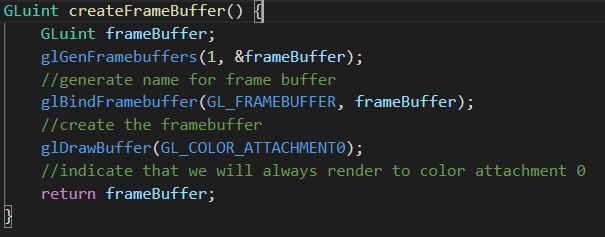
\includegraphics[width= 1
	\textwidth]{images/FBO1.png}
	\caption{Method for the creation of the frame buffer.}
\end{figure} 

\noindent
So I defined two methods for creating texture attachment, one for colour and one for depth attachment. They are just a simple generation of a texture with a new "glFramebufferTexture" statement. (I only inserted the screenshot of the colour attachment since they are pretty much the same).

\begin{figure}[hbt!]
	\centering
	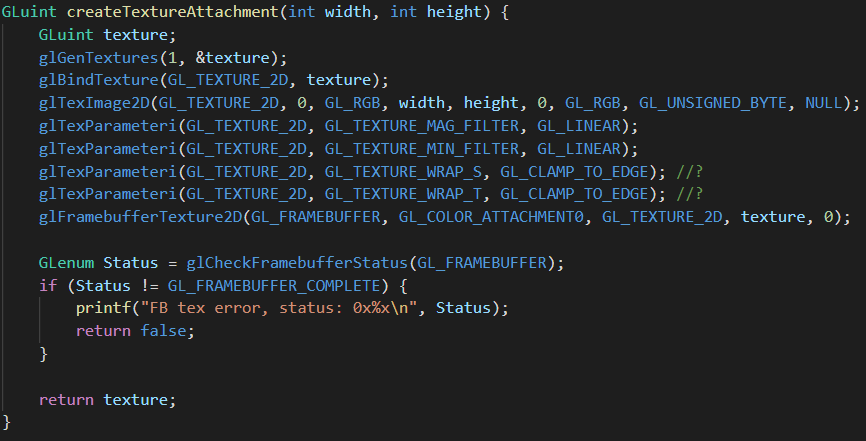
\includegraphics[width= 0.9
	\textwidth]{images/FBO2.png}
	\caption{Method for the creation of the texture.}
\end{figure} 

Last I defined a method to create the depth buffer. 

\begin{figure}[hbt!]
	\centering
	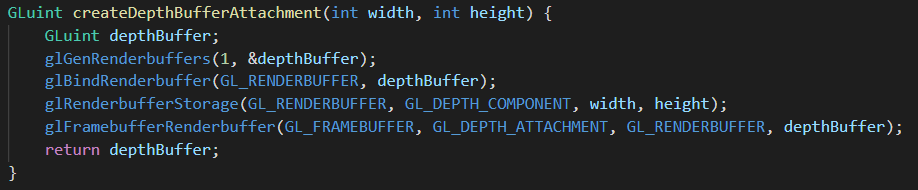
\includegraphics[width= 1
	\textwidth]{images/FBO4.png}
	\caption{Method for the creation of depth buffer.}
\end{figure} 

\noindent
Finally I created two methods, one to bind the frame buffer and one to unbind it so that I can switch from the normal frame buffer to the one created by me. I stored two frame buffers in this class, one for reflection and one for refraction. Basically I'll render the scene and create my own texture that will be used by the main render to apply it to the water.

\subsection{Clipping plane}
For both refraction and reflection textures, you don't need to render the whole scene. Actually I need the one above the surface for the reflection and the one under the water for refraction. So I defined the clipping plane which allowed me to render only a part of the scene and obviously it is positioned at the same level of the water. \\
After enabling a clipping plane (\textbf{glEnable(GL\textunderscore CLIP\textunderscore DISTANCE0)}) in the main rendering, I use the \textbf{gl\textunderscore ClipDistance[0]} variable in the shaders to define which vertex should be clipped. If this distance is positive, I should render this vertex, if negative no. To calculate it, I simply use the dot product of the world position (model matrix * position) and the horizontal plane, whose equation is \textbf{vec4}(0, -1/+1, +/-waterHeight). The Y component will be +1 if we want to clip the lower part (reflection) or -1 if we want to clip the upper part (refraction)

\newpage

\begin{figure}[hbt!]
	\centering
	\subfloat[\centering Clipping the below part.]{{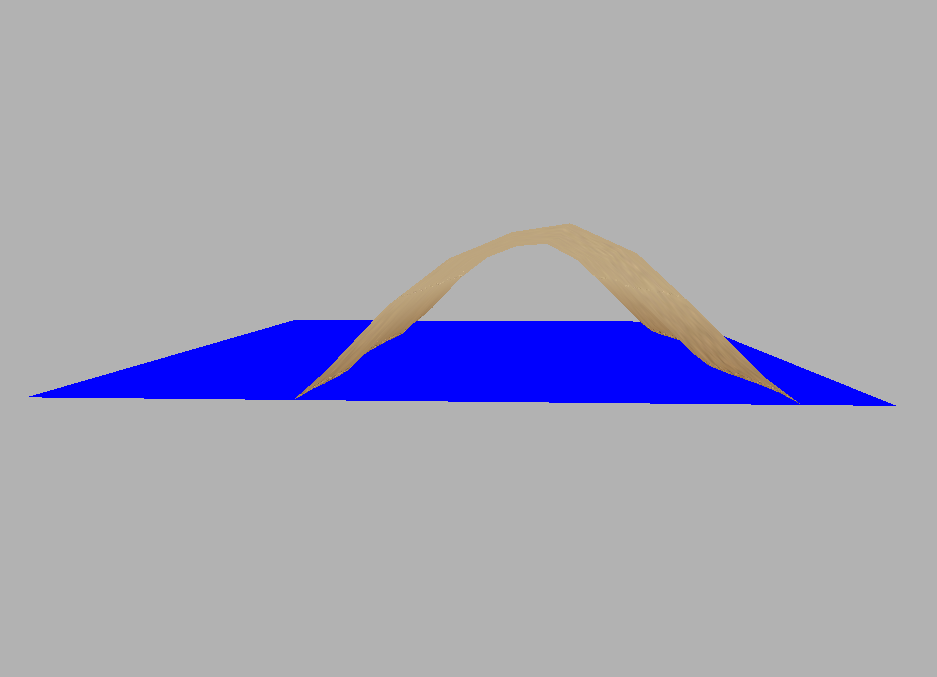
\includegraphics[width=6.3cm]{images/Water1.png}}}%
	\qquad
	\subfloat[\centering Clipping the above part.]{{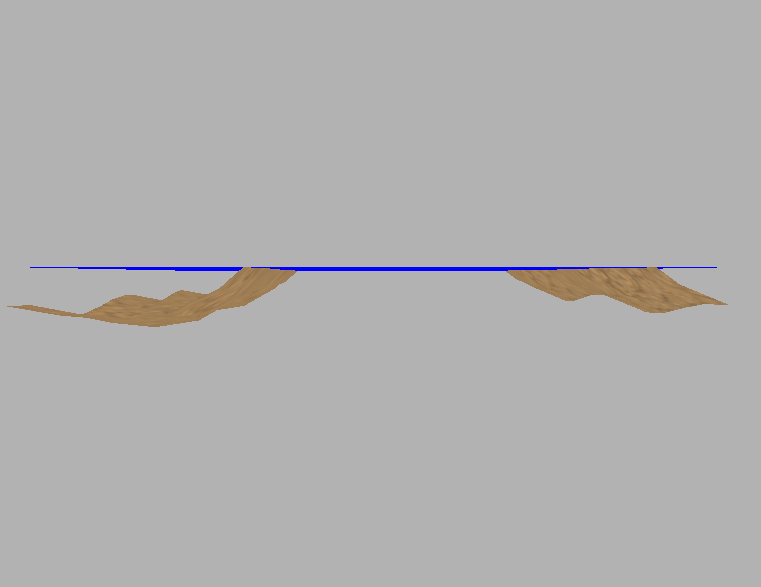
\includegraphics[width=6.3cm]{images/Water2.png} }}%
	\caption{}
\end{figure}

\subsection{Projective texture mapping}
To apply the texture to the plane, I used \textbf{projective texture mapping} that is a texture mapping method that allows you to project a textured image onto a scene. I needed to find the correct UV coordinate and for that I just found the screen space coordinate on the water coordinates and I can use those exactly to sample the texture. Basically I need to calculate the normalized device coordinates and I can do it using the perspective division. I just need to divide the clip space component (projection matrix * view matrix * model matrix * position) into its \textbf{W} component and then divide by 2 and add 0.5 to find the correct coordinate system .

\begin{equation}
newCoord = vec2(clipspace.xy / clipspace.w) / 2.0 + 0.5)		
\end{equation}

\noindent
Now I can sample the refraction and the reflection by using the X and Y components as texture coordinates.
I also need to mention that the rendering for the reflection texture is done with the camera reversed and shifted slightly down to give the reflection effect. On the other hand, no changes are applied to refraction rendering.

\newpage

\begin{figure}[hbt!]
	\centering
	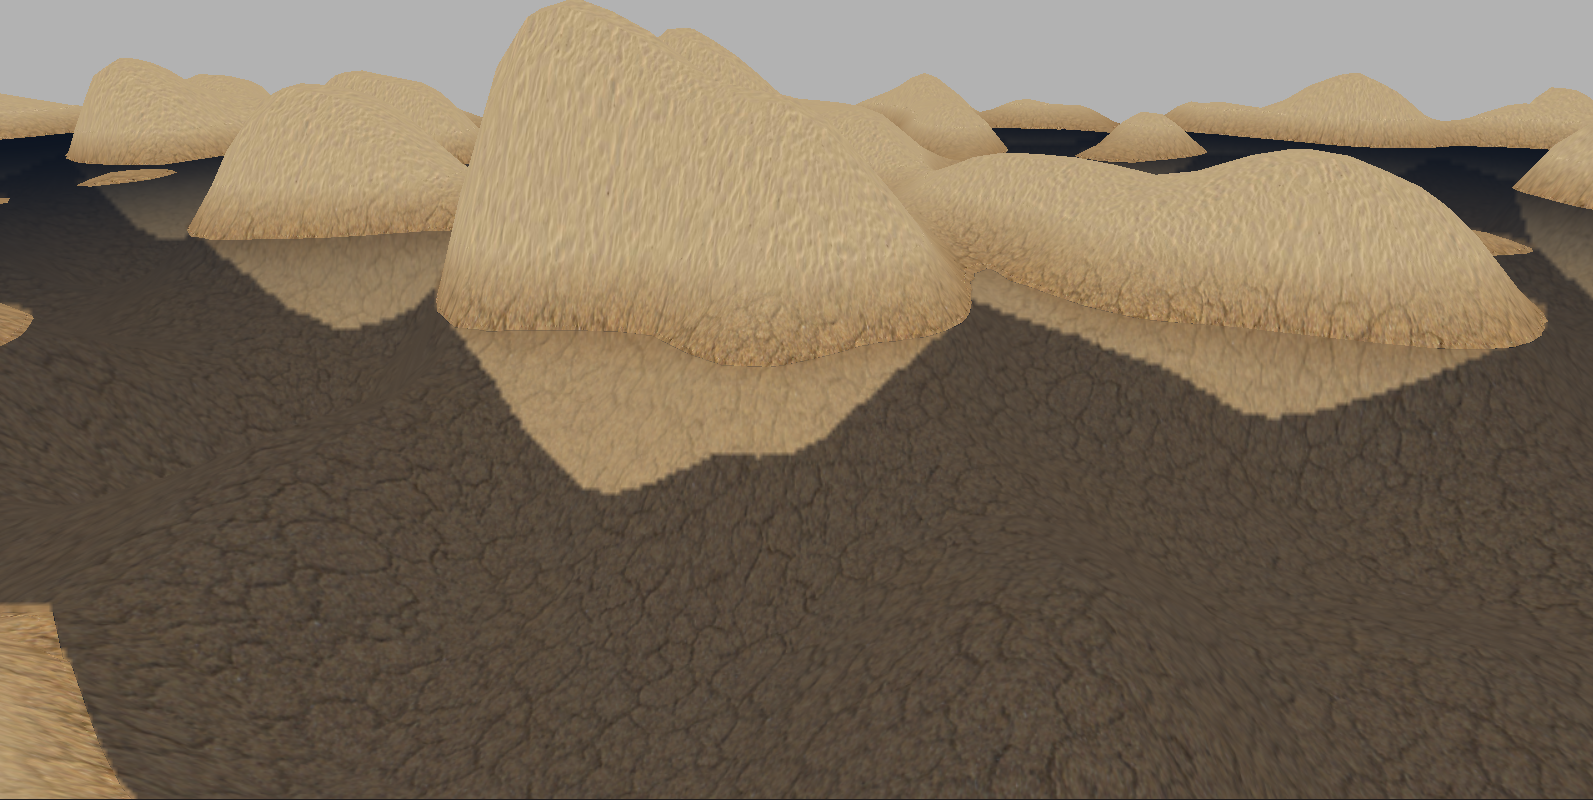
\includegraphics[width= 1
	\textwidth]{images/Water3.png}
	\caption{Reflection and Refraction texture mixed.}
\end{figure} 

\subsection{DuDv Maps}
To create a more realistic water, I used a particular texture to distort the water.

\begin{figure}[hbt!]
	\centering
	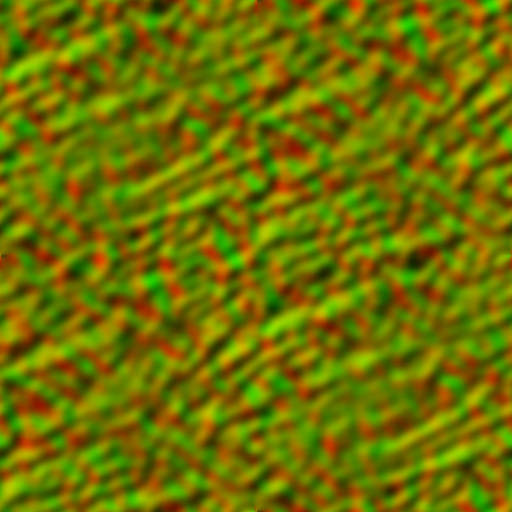
\includegraphics[width= 0.5
	\textwidth]{../textures/plane/waterDUDV.png}
	\caption{DuDv texture.}
\end{figure} 

\noindent
Basically, I sampled this new texture and used these coordinates to change the value of the previously calculated texture coordinates, in the x component and in the y component. To change the coordinates over time, I create a uniform variable called waterMovement to change the position of the coordinates at each frame. Since the value of our dudv texture is always positive, I applied a conversion to create value from -1 and 1, multiplied by 2 and subtracted by 1. After adding the distortion, I clamped the result to have a value between 0 and 1.

\begin{figure}[hbt!]
	\centering
	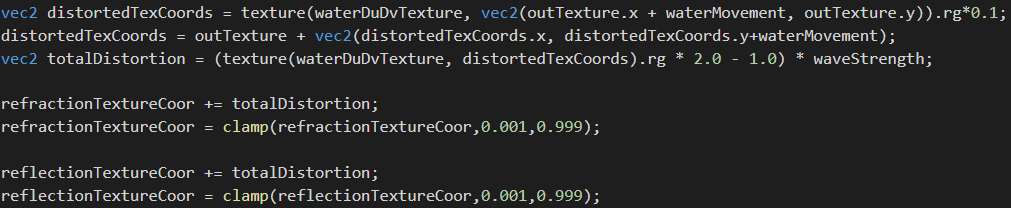
\includegraphics[width= 1
	\textwidth]{images/TextDist.png}
	\caption{\textbf{waterShader.frag} distortion part.}
	\label{fig::distortion}
\end{figure}

\begin{figure}[hbt!]
	\centering
	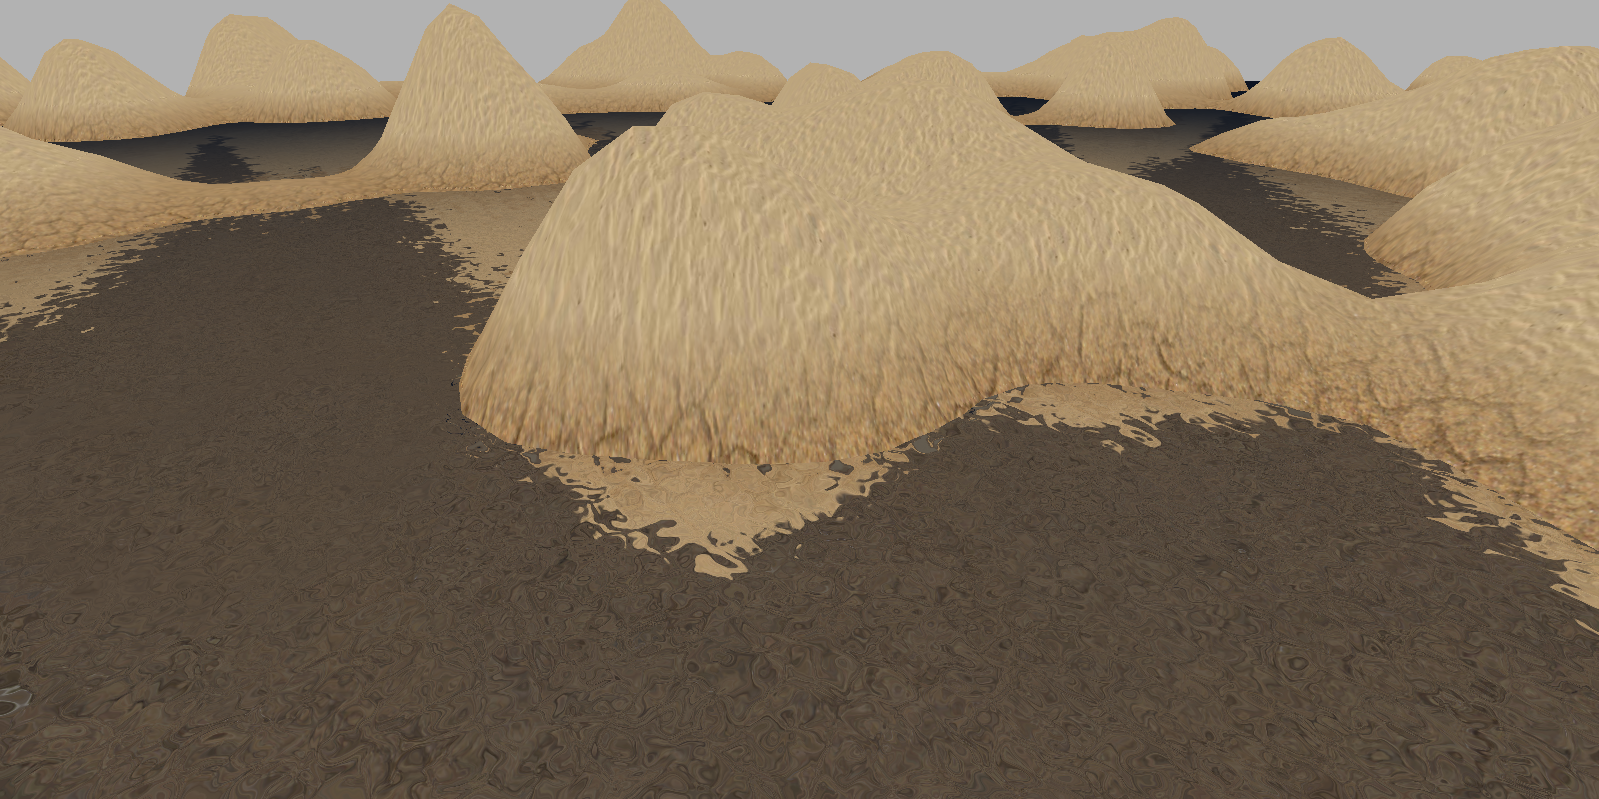
\includegraphics[width= 1
	\textwidth]{images/Water4.png}
	\caption{Water distortion.}
\end{figure}

\subsection{Normal map}
I want to simulate a light effect on the surface of the water. To do this I used a normal map which is similar to the dudv map above. 

\newpage

\begin{figure}[hbt!]
	\centering
	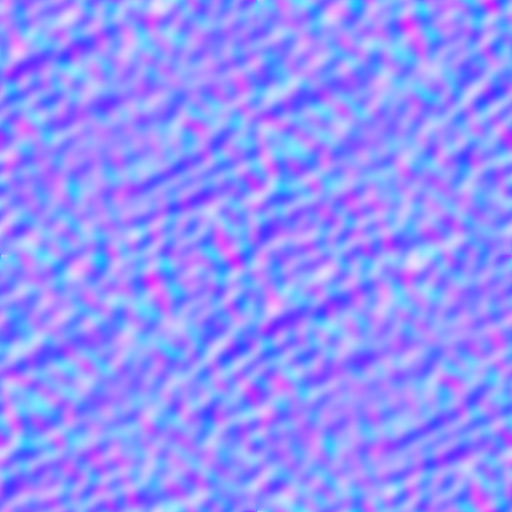
\includegraphics[width= 0.5
	\textwidth]{../textures/plane/normalMap.png}
	\caption{Normal texture.}
\end{figure} 

\noindent
In the shader, after sampling the texture, I calculated the normal vector using the red component for the X, the blue component for the Y and the green component for the Z. We want the Y component to always be positive, while the X and Z they can also be negative. So we multiplied the two coordinates by 2 and subtracted by 1 as we did before. After that I normalized the vector.

\begin{equation}
\text{vec3 normal} = vec3(normalMap.r * 2 - 1, normalMap.b, normalMap.g * 2 - 1)		
\end{equation}

\noindent
Next I passed as uniform the position of the camera, the position of the light and I added a few more parameters to create the specular lighting on the water like \textbf{shineDamper} to determine the distance from where the camera will see any difference in the brightness of the surface and \textbf{reflectivity} which determined the amount of reflected light.
Then I calculated the vector from the light to the vertex using the world position (model * position) and the vector from the world position to the camera.

\begin{equation}
\text{vec3 fromLightVector} = normalize(WorldPosition - lightPos);
\end{equation}

\begin{equation}
\text{vec3 viewVector} = normalize(cameraPos - WorldPosition);
\end{equation}

\noindent
Now I can first calculate the reflection of \textbf{fromLightVector} with the normal, then calculate the dot product of \textbf {viewVector} and the reflected light to understand how bright the surface will be at that point. After that we had to use the pow function between the dot product calculated earlier and the \textbf{shineDamper}. Finally, we can multiply the light colour (passed as uniform), the calculated specular illumination and the reflectivity.

\begin{figure}[hbt!]
	\centering
	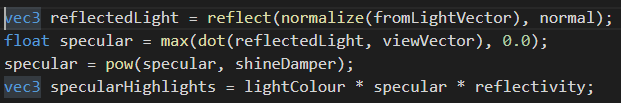
\includegraphics[width= 1
	\textwidth]{images/Light.png}
	\caption{Specular lighting code.}
	\label{fig::highlights}
\end{figure} 

\begin{figure}[hbt!]
	\centering
	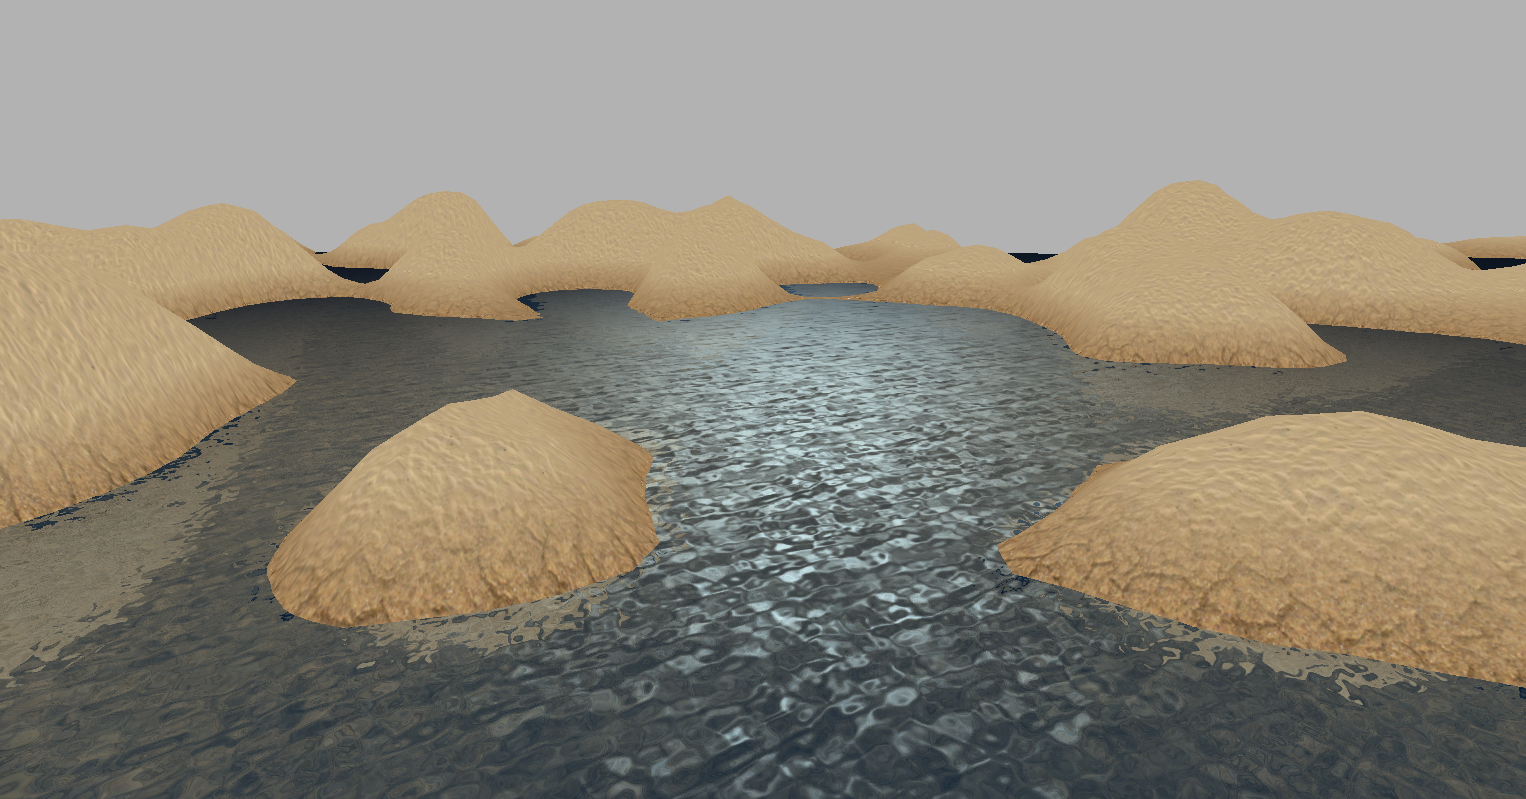
\includegraphics[width= 1
	\textwidth]{images/Water5.png}
	\caption{Specular lighting}
\end{figure} 

\subsection{Soft edges}
There is one last problem to be solved and it is caused by the distortion, in fact, there are rendered parts that should not be in the water.

\newpage

\begin{figure}[hbt!]
	\centering
	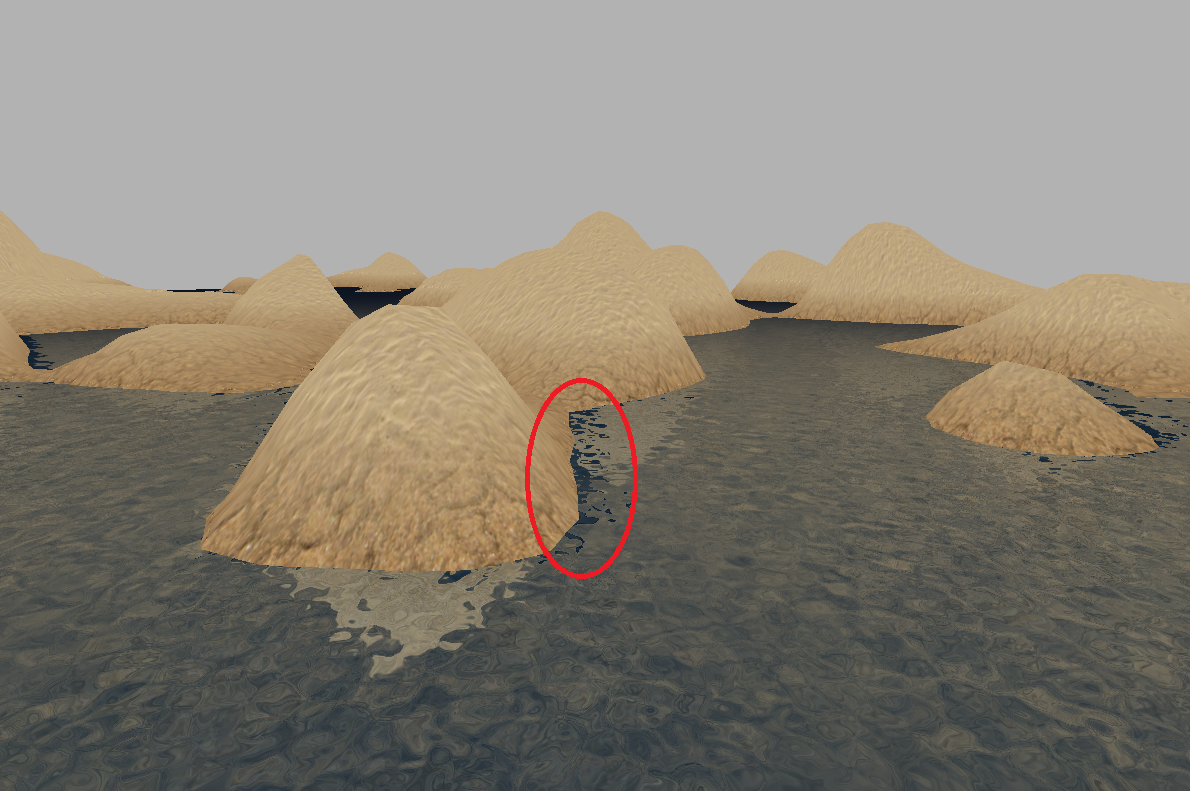
\includegraphics[width= 0.9
	\textwidth]{images/Water6.png}
	\caption{Picture that shows the problem}
\end{figure} 

\noindent
I want to calculate the distance between the bottom of the water and the water plane to the camera in the shader.

\begin{figure}[hbt!]
	\centering
	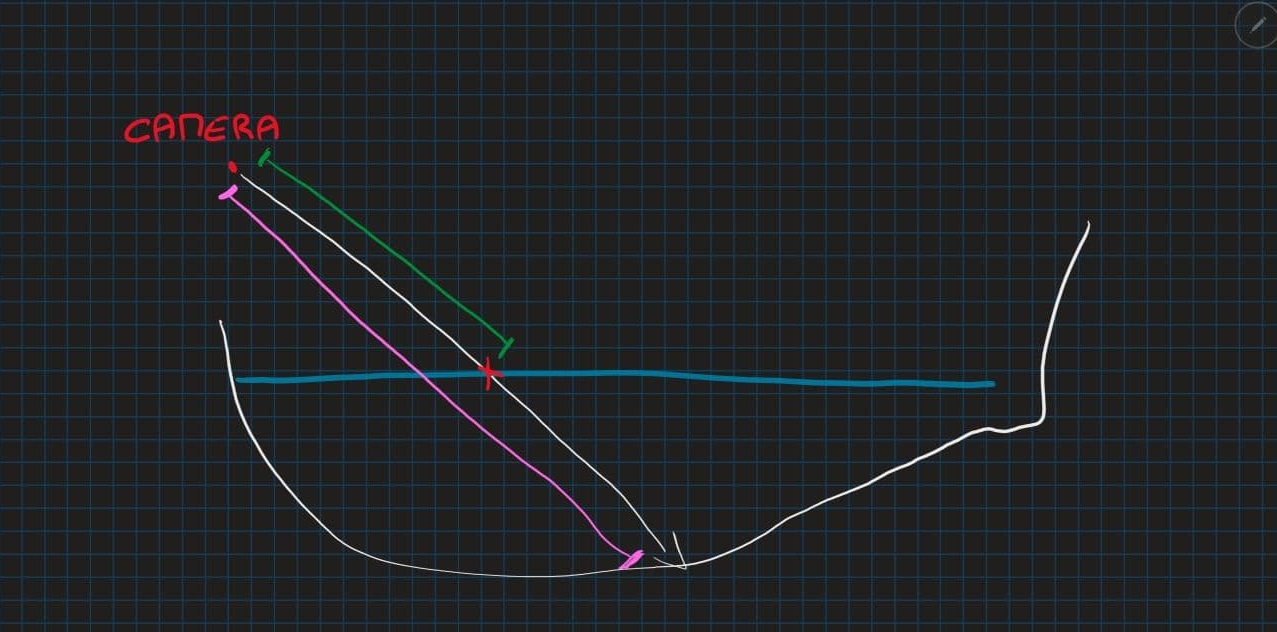
\includegraphics[width= 0.9
	\textwidth]{images/Water7.jpg}
	\caption{We want the subtraction between pink line and green line}
\end{figure} 

\noindent
To calculate the distance from the bottom of the water I will use the refractive depth texture calculated in the FBO. However, the \textbf{r} component of the depth texture gives us a value between 0 and 1. To convert it to a distance I used a formula that uses the far and near plane.
To calculate the distance from the plane I can use an OpenGl variable called \textbf{gl\textunderscore FragCoord}, then take the Z component that gives us the depth of this fragment and then apply the same formula as above. Finally I subtract the two values.

\begin{figure}[hbt!]
	\centering
	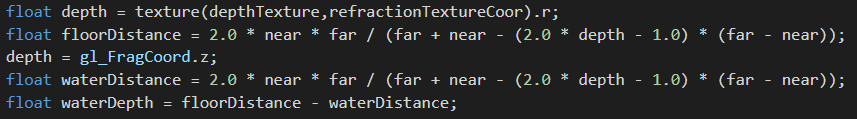
\includegraphics[width= 1
	\textwidth]{images/Water8.png}
	\caption{Code of the above passage.}
\end{figure} 

\begin{figure}[hbt!]
	\centering
	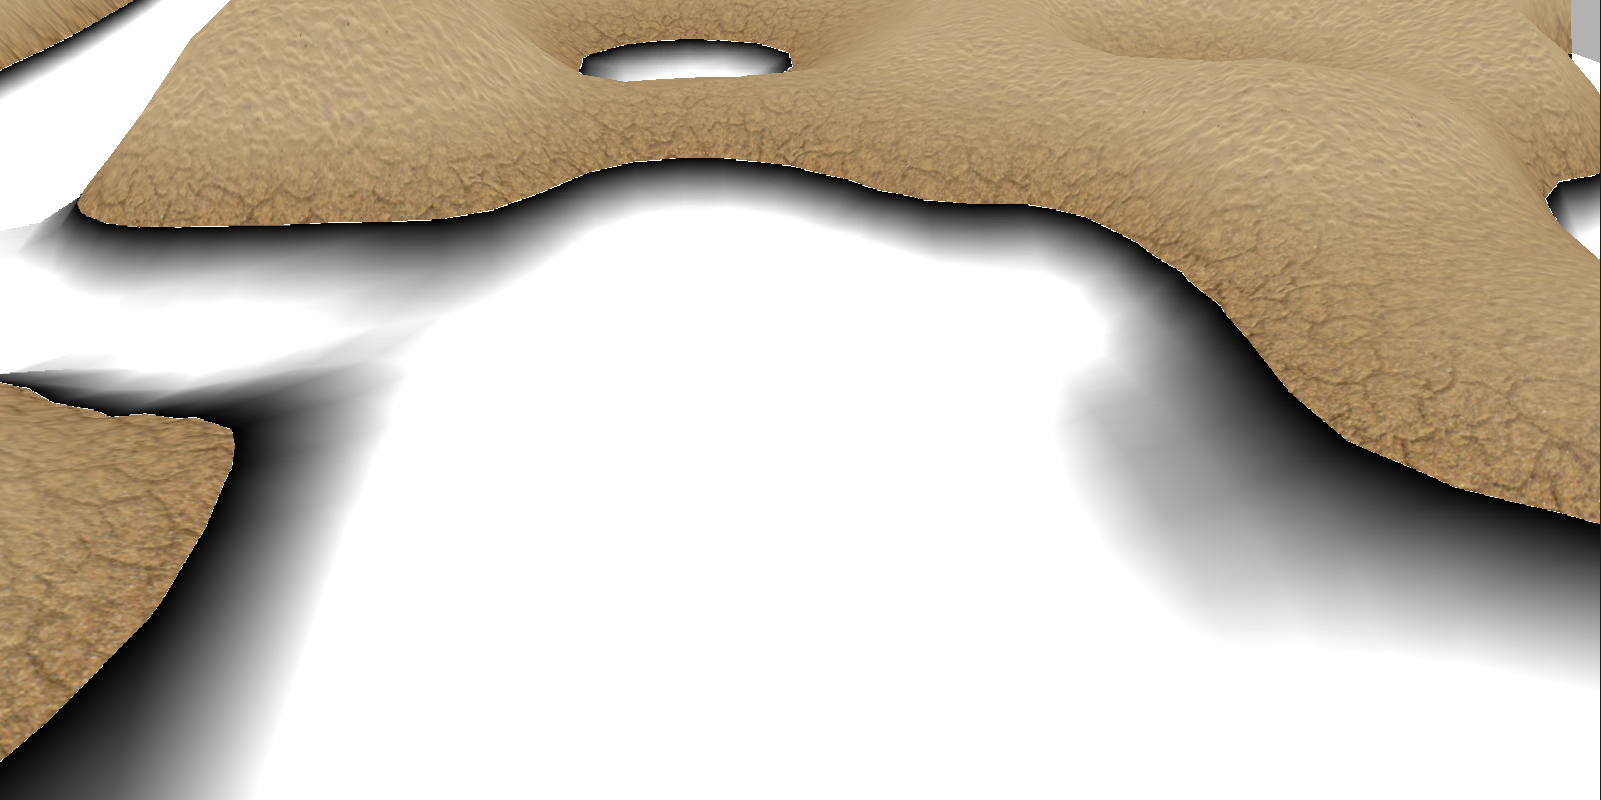
\includegraphics[width= 1
	\textwidth]{images/Water9.png}
	\caption{Water depth values applied in the water.}
\end{figure}

\noindent
Now we want to use this information to change the water near the edges. When the depth value is 0, the water is transparent. So the closer you get to the value 1, the less transparent the water is. After the value 1 there is no transparency.
Basically I just need to clamp my water depth (divided by a factor that determines how long the transition from 0 to 1 takes) and multiply it by the \textbf{totalDistortion} value in the figure \ref {fig::distortion} and the value \textbf{specularHighlights} in figure \ref {fig::highlights}.

\newpage

\begin{figure}[hbt!]
	\centering
	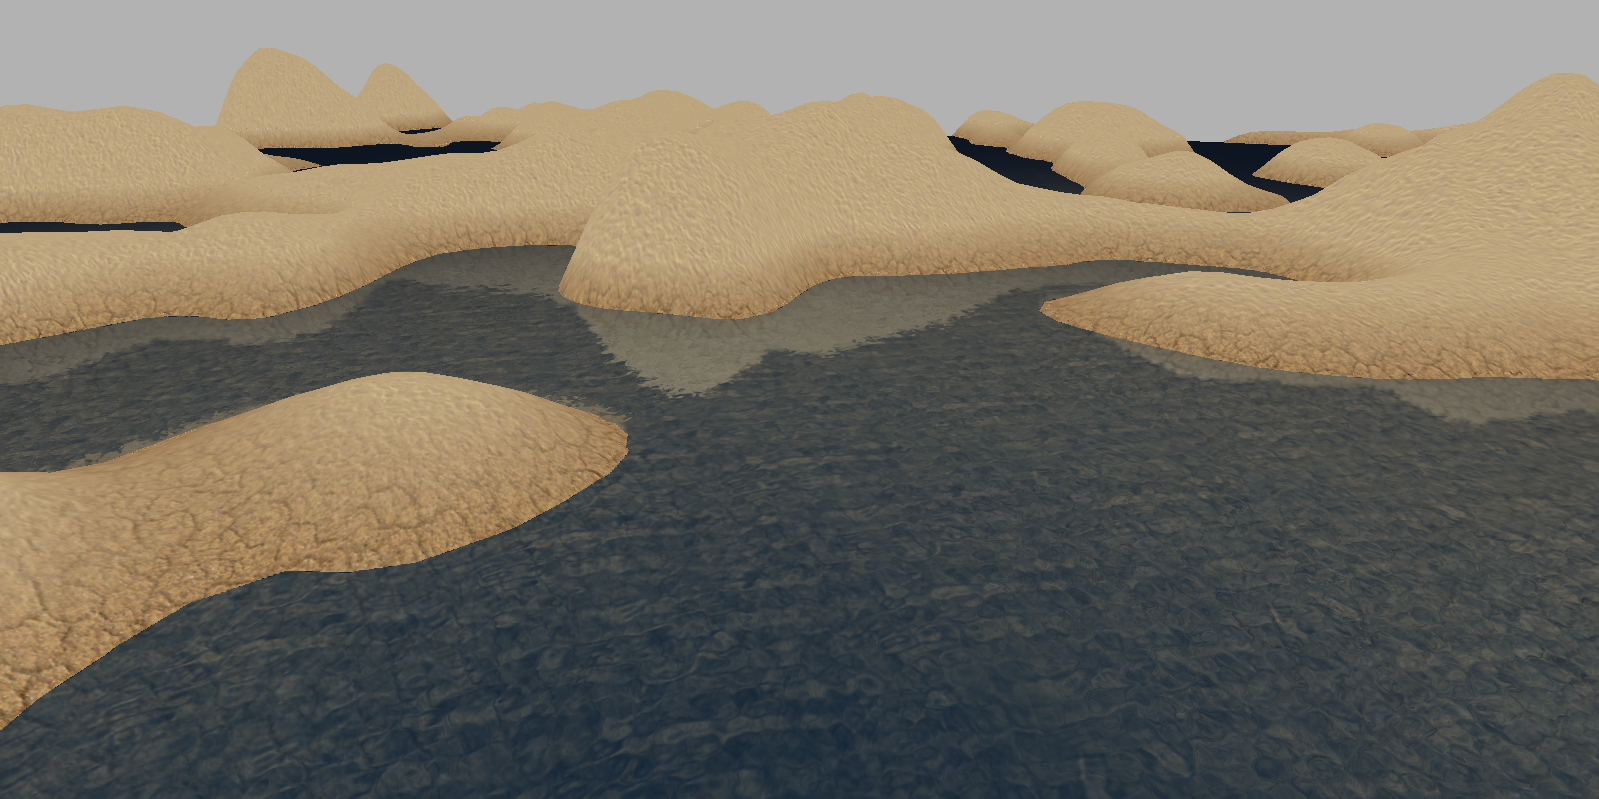
\includegraphics[width= 1
	\textwidth]{images/Water10.png}
	\caption{Water result after all stages.}
\end{figure}

\newpage

\section{Cube Map}
I used a cube map to create the sky. One of the images I chose, contains a moon to give the illusion that the light comes from there (the light source is indeed in the same direction).

\begin{figure}[hbt!]
	\centering
	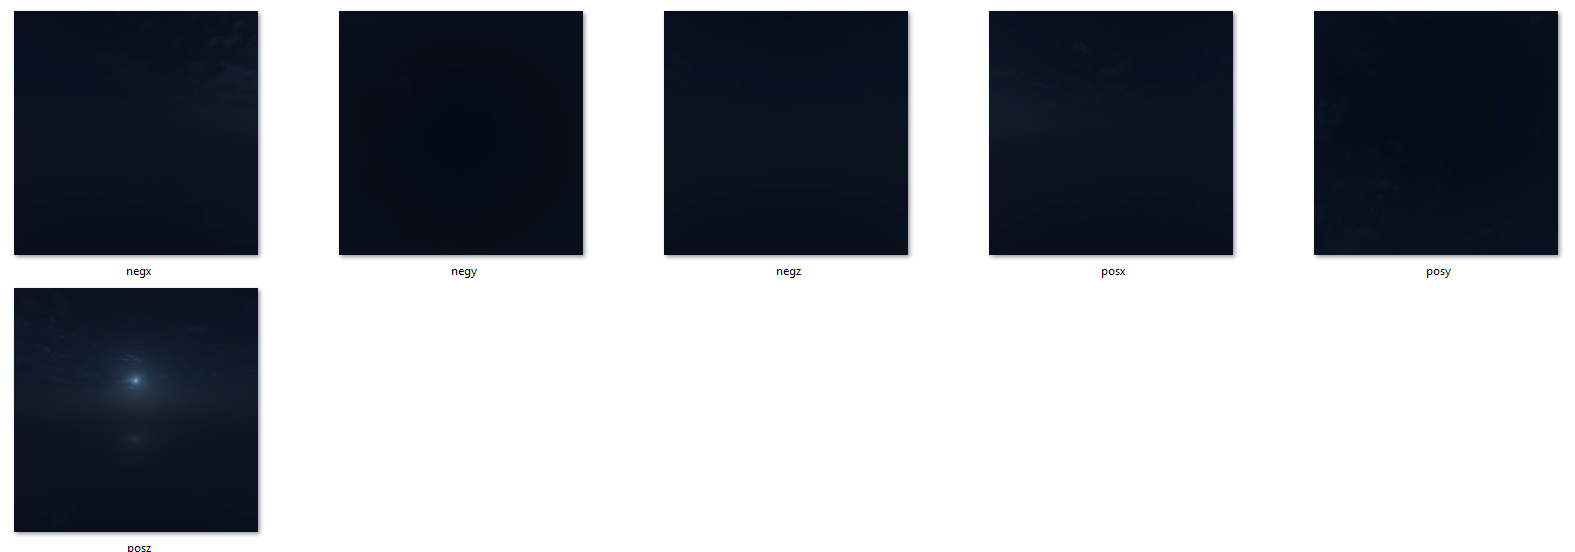
\includegraphics[width= 1
	\textwidth]{images/Sky.png}
	\caption{Images used for the cube map.}
\end{figure}

\begin{figure}[hbt!]
\centering
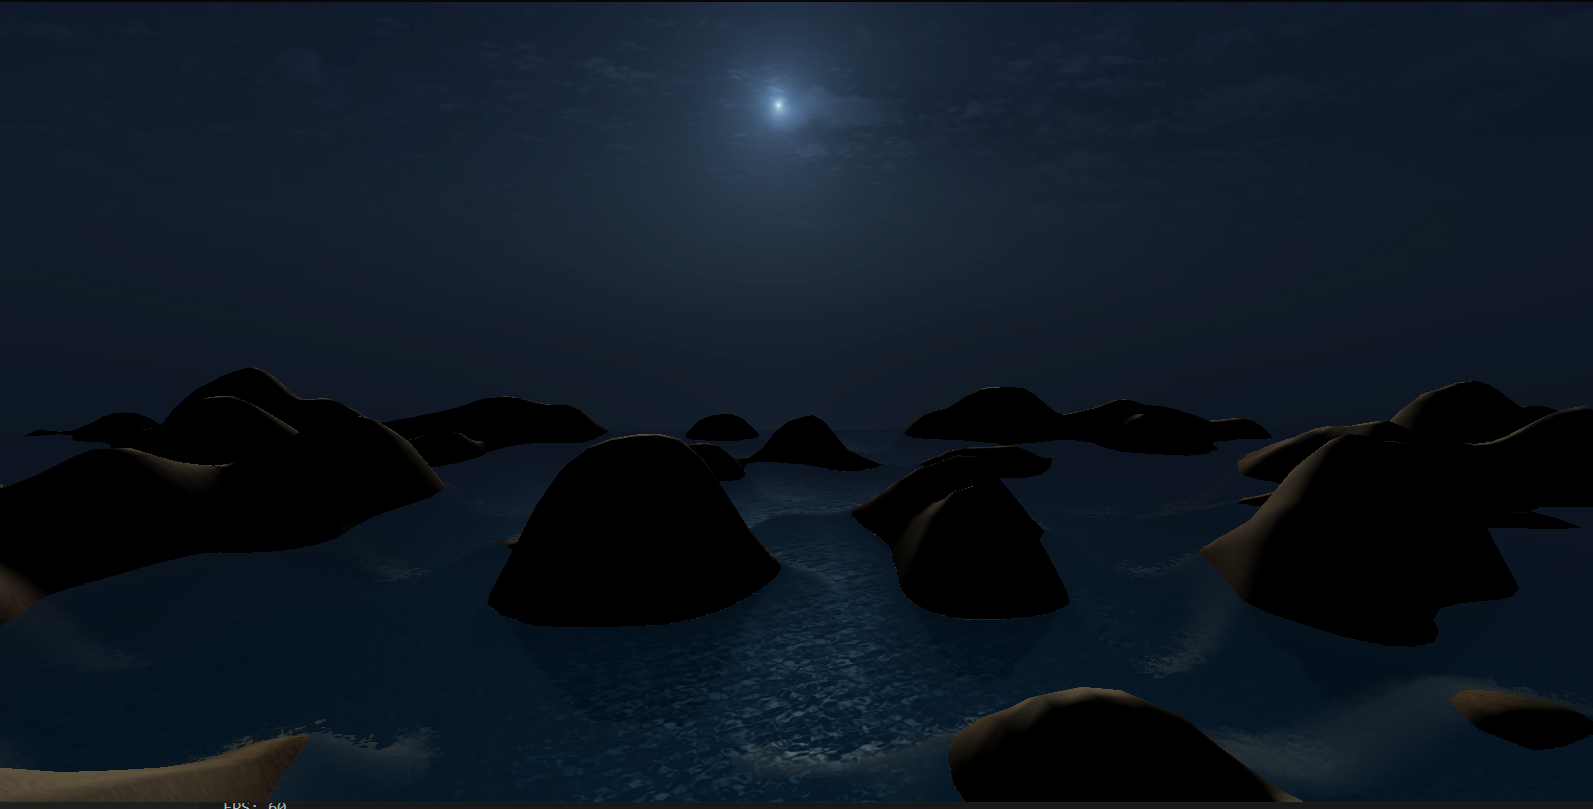
\includegraphics[width= 1
\textwidth]{images/Sky2.png}
\caption{Cube map applied.}
\end{figure}

\subsection{Fog}
Right now I can see the movement of the cells. To avoid this I need to create a fog. The general idea is to blend objects with the colour of the sky, depending on how far they are from the camera. Near objects will have their normal colour, distant ones will have the same colour as the sky, and the objects in the middle will have a mixed colour. To do this I introduced a variable called \textbf{visibility} used in each shader, whose value goes from 0 (object in the fog) to 1 (normal colour). I used an exponential formula to calculate the visibility which has two parameters: \textbf{density} and \textbf{gradient}. The first represents the thickness of the fog and increasing this value will decrease the overall visibility of the scene. The second determined how quickly visibility decreases with distance, and increasing this value makes the transition from 0 visibility to full visibility much smaller. To get the distance from the camera I used the built-in GLSL length function on the \textbf{positionRelativeToCam} variable (view matrix * model matrix * position).

\begin{figure}[hbt!]
	\centering
	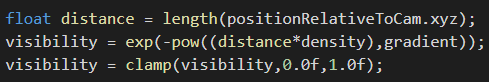
\includegraphics[width= 1
	\textwidth]{images/fog.png}
	\caption{Code for the fog visibility calculation.}
\end{figure}

\noindent
After calculating the visibility I mixed the color value with the fog color (usually the sky color) using the visibility factor in the fragments shader.

\begin{equation}
\text{FragColour} = mix(vec4(fogColour,1), FragColour, visibility);
\end{equation}

\newpage

\begin{figure}[hbt!]
	\centering
	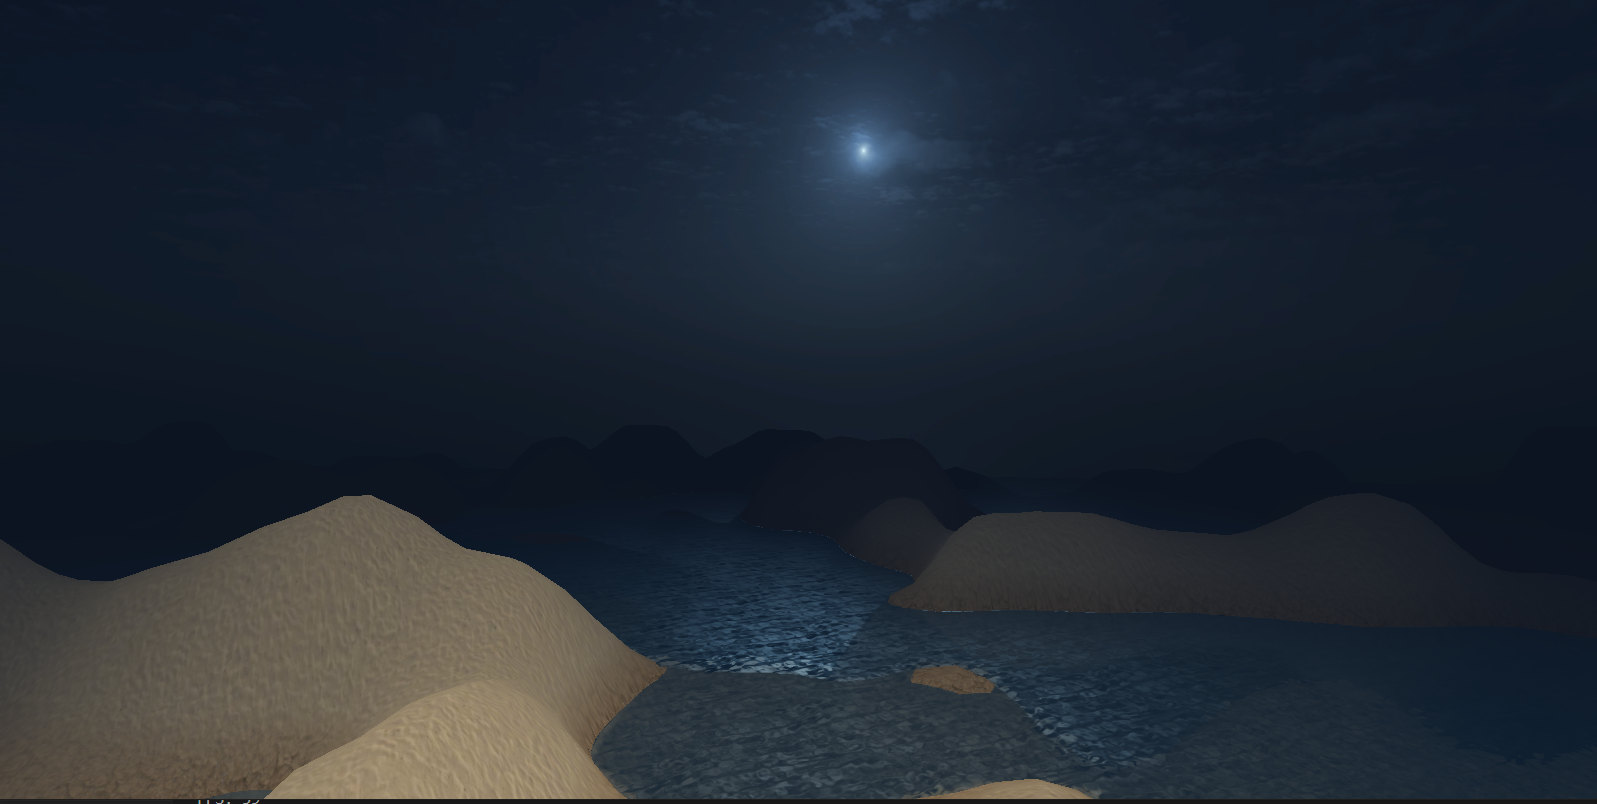
\includegraphics[width= 0.9
	\textwidth]{images/fog1.png}
	\caption{Fog with fixed colour.}
\end{figure}

\noindent
Perhaps in the image it is not very visible but there is still a problem. Fog is a fixed colour, but the sky has several. In fact, I can still see the movement of the terrain. The solution is to blend the horizon of the cube map with the colour of the fog. I have defined a lower and an upper limit. As before, below the lower limit, the cube map will have the colour of fog, above the upper limit it will be normal, and in the middle it will be mixed.

\begin{figure}[hbt!]
	\centering
	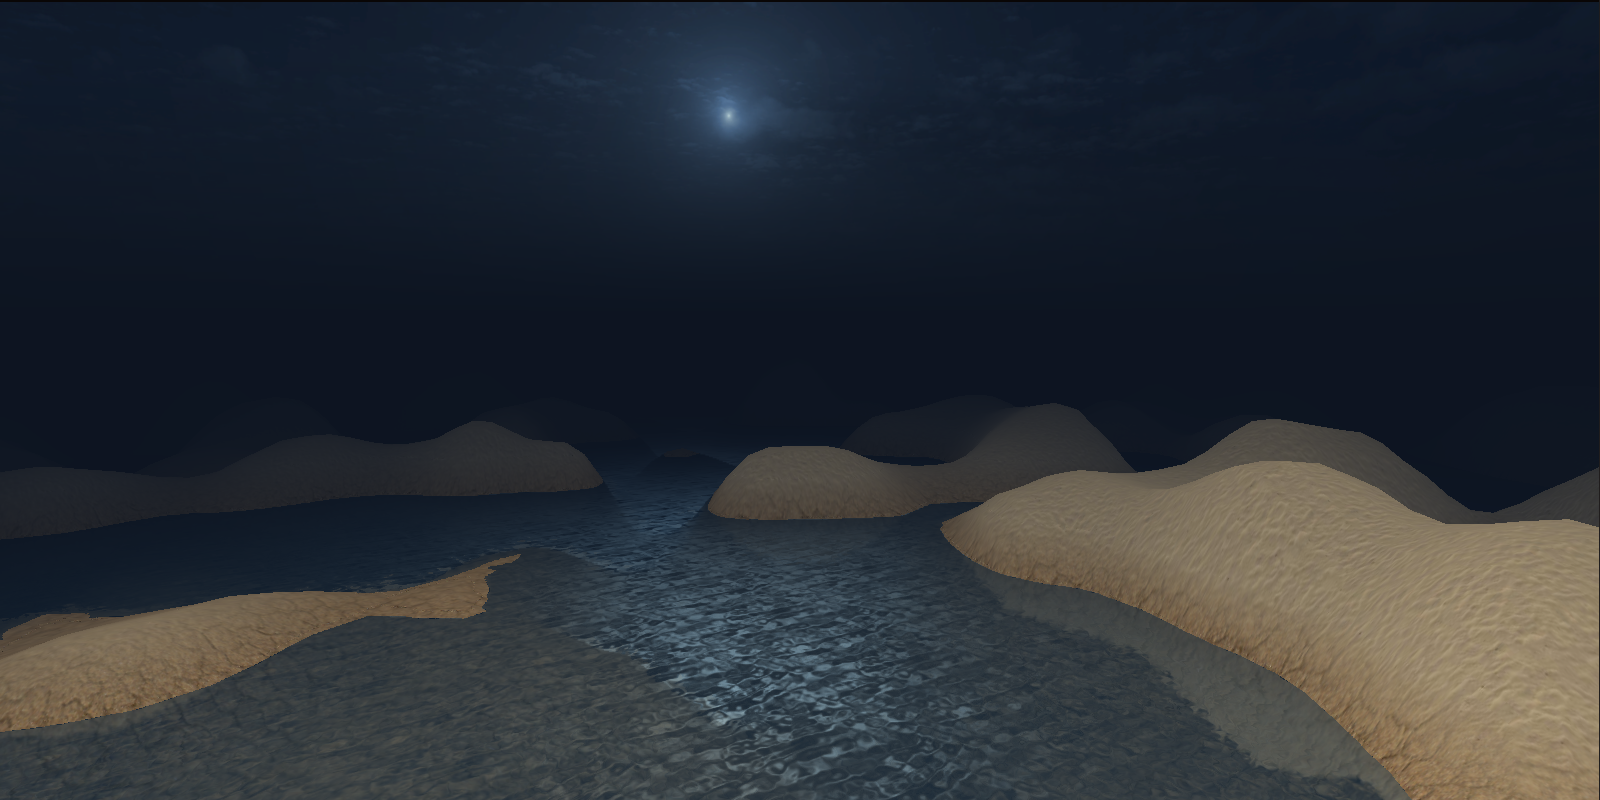
\includegraphics[width= 0.9
	\textwidth]{images/fog2.png}
	\caption{Final fog result.}
\end{figure}

\newpage

\section{Other elements}
I decided to decorate the scene with other elements, in particular with trees and cactus. To keep things simple, I randomly assign one of the two models to each cell above the water. The only difficult thing is to calculate the height of the ground to position the object correctly.

\begin{figure}[hbt!]
	\centering
	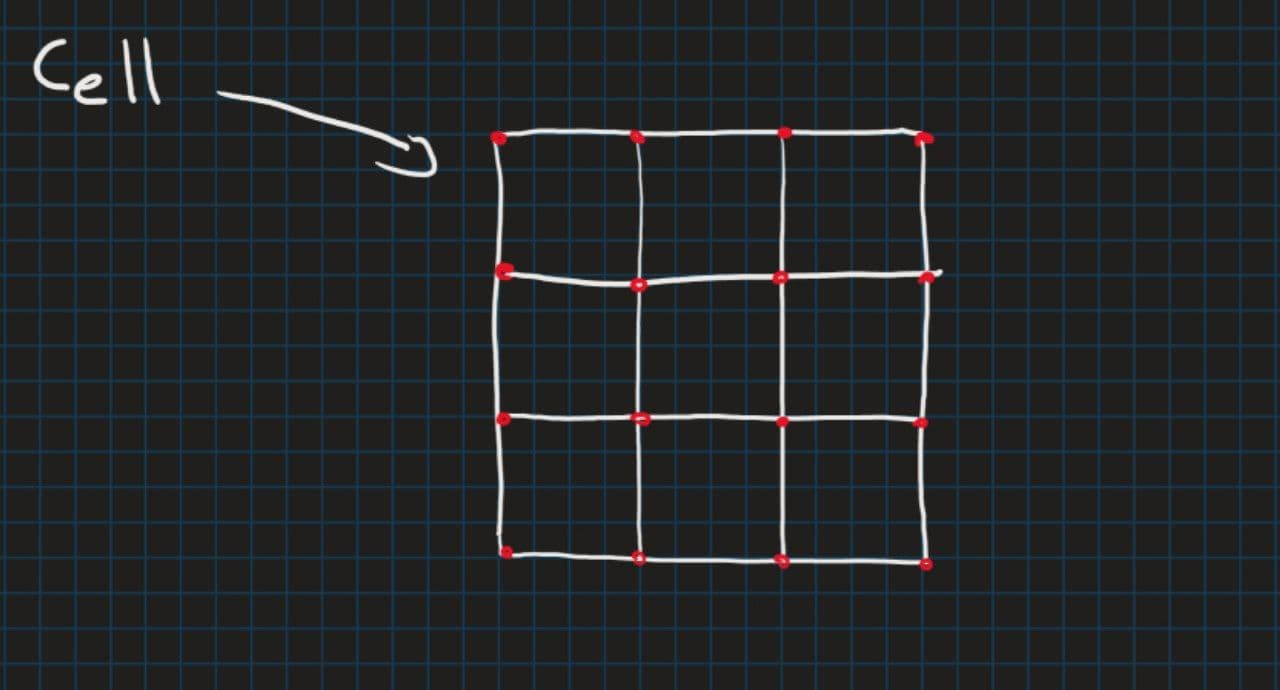
\includegraphics[width= 0.75
	\textwidth]{images/object.jpg}
	\caption{Grid square of a cell.}
\end{figure}

\noindent
Given a position within a cell, I need to calculate the height of that point. First I need to find the size of a grid square. I divided the size of a cell by the number of vertices subtracted by one. For example in the image above there are four vertices and with a size of 500, the size of the grid square is 500/3. Now I can calculate which square of a grid is the object in by dividing the X and Y coordinates of the object's position with the grid size and floor the result. Now I want to calculate the coordinates of the object in that grid square. To do this I apply the module operator between the position and size of the square and then divide it by the size of the square. Basically now I have the coordinate inside a square from 0 to 1. To understand which triangles is the object in, I checked the X coordinate and I saw if it is less than or greater than 1 - Z. Finally I have my triangle and I have the height of the vertices and I can calculate the height of my points in several possible ways, for example using the barycentric interpolation.
After doing this, we can easily place the different objects at the right height.

\newpage

\begin{figure}[hbt!]
	\centering
	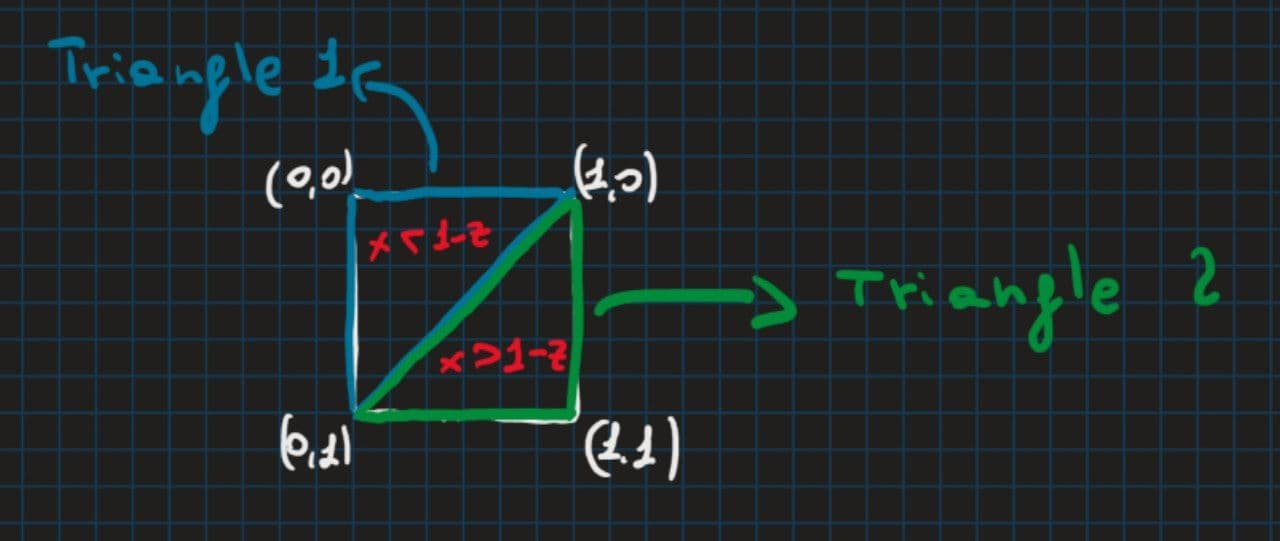
\includegraphics[width= 1
	\textwidth]{images/object2.jpg}
	\caption{Grid square triangles division.}
\end{figure}

\begin{figure}[hbt!]
	\centering
	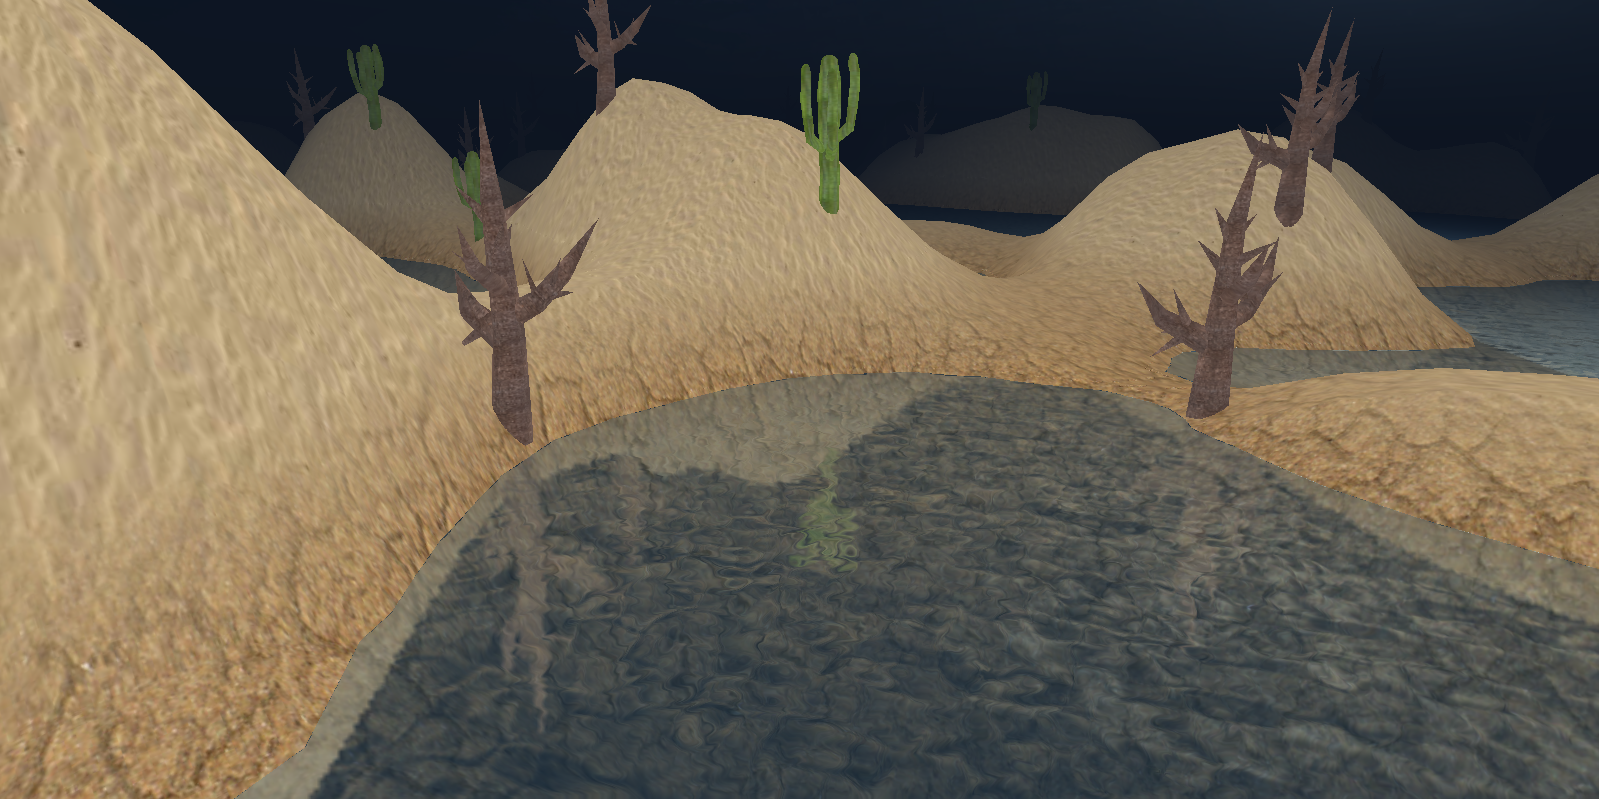
\includegraphics[width= 1
	\textwidth]{images/object3.png}
	\caption{Trees and cactus positioned.}
\end{figure}

\newpage

\section{Performance}
The machine I used to develop the project has these characteristics:

\begin{itemize}
	\item Processor: Intel Core I7-7700HQ CPU 2.8 GHz.
	\item Ram: 16 GB.
	\item Included Graphics card: Intel HD Graphics 630.
	\item Graphics card: NVIDIA GeForce GTX 1050, 4GB.
	\item Hard disk: 1024 HDD, 256 SSD. 
\end{itemize}

\noindent
Let's now analyze the performance of the project based on the different value of the terrain. I leave the function that calculates the FPS value.

\begin{figure}[hbt!]
	\centering
	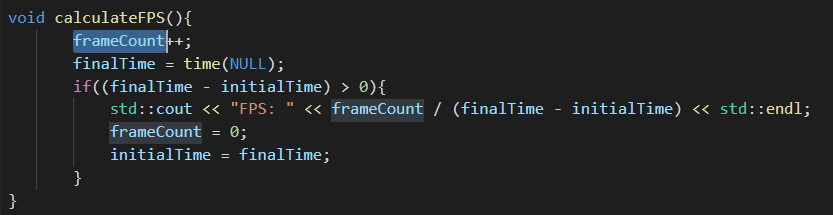
\includegraphics[width= 1
	\textwidth]{images/fps2.png}
	\caption{FPS calculation.}
\end{figure}

\noindent
I will only customize the Terrain mesh, as the water is just a plane with 2 vertices per row / column (4 vertices in total in this case) and I don't need more (the size is the same as a cell) and trees and cactus are imported from a model.

\subsection{4 vertices each row/column}
With 4 vertices, each cell has 16 vertices in total. I have a steady 60 FPS, but the terrain feels too polygonal and isn't very good.

\newpage

\begin{figure}[hbt!]
	\centering
	
	\noindent\makebox[\textwidth]{\includegraphics[width=1.4\textwidth,height=0.5\textheight]{images/fps3.png}}%
	
	\caption{Scene with FPS below. (16-vertices for cell, 441 cells, size 2000, height 24000)}
\end{figure} 

\subsection{8 vertices each row/column}
With 8 vertices, each cell has 64 vertices. If we use 441 cells, we have a total of 28224 vertices. With a cell size of 500, the scene is rendered with a range between 58 and 60 FPS.

\newpage

\begin{figure}[hbt!]
	\centering
	
	\noindent\makebox[\textwidth]{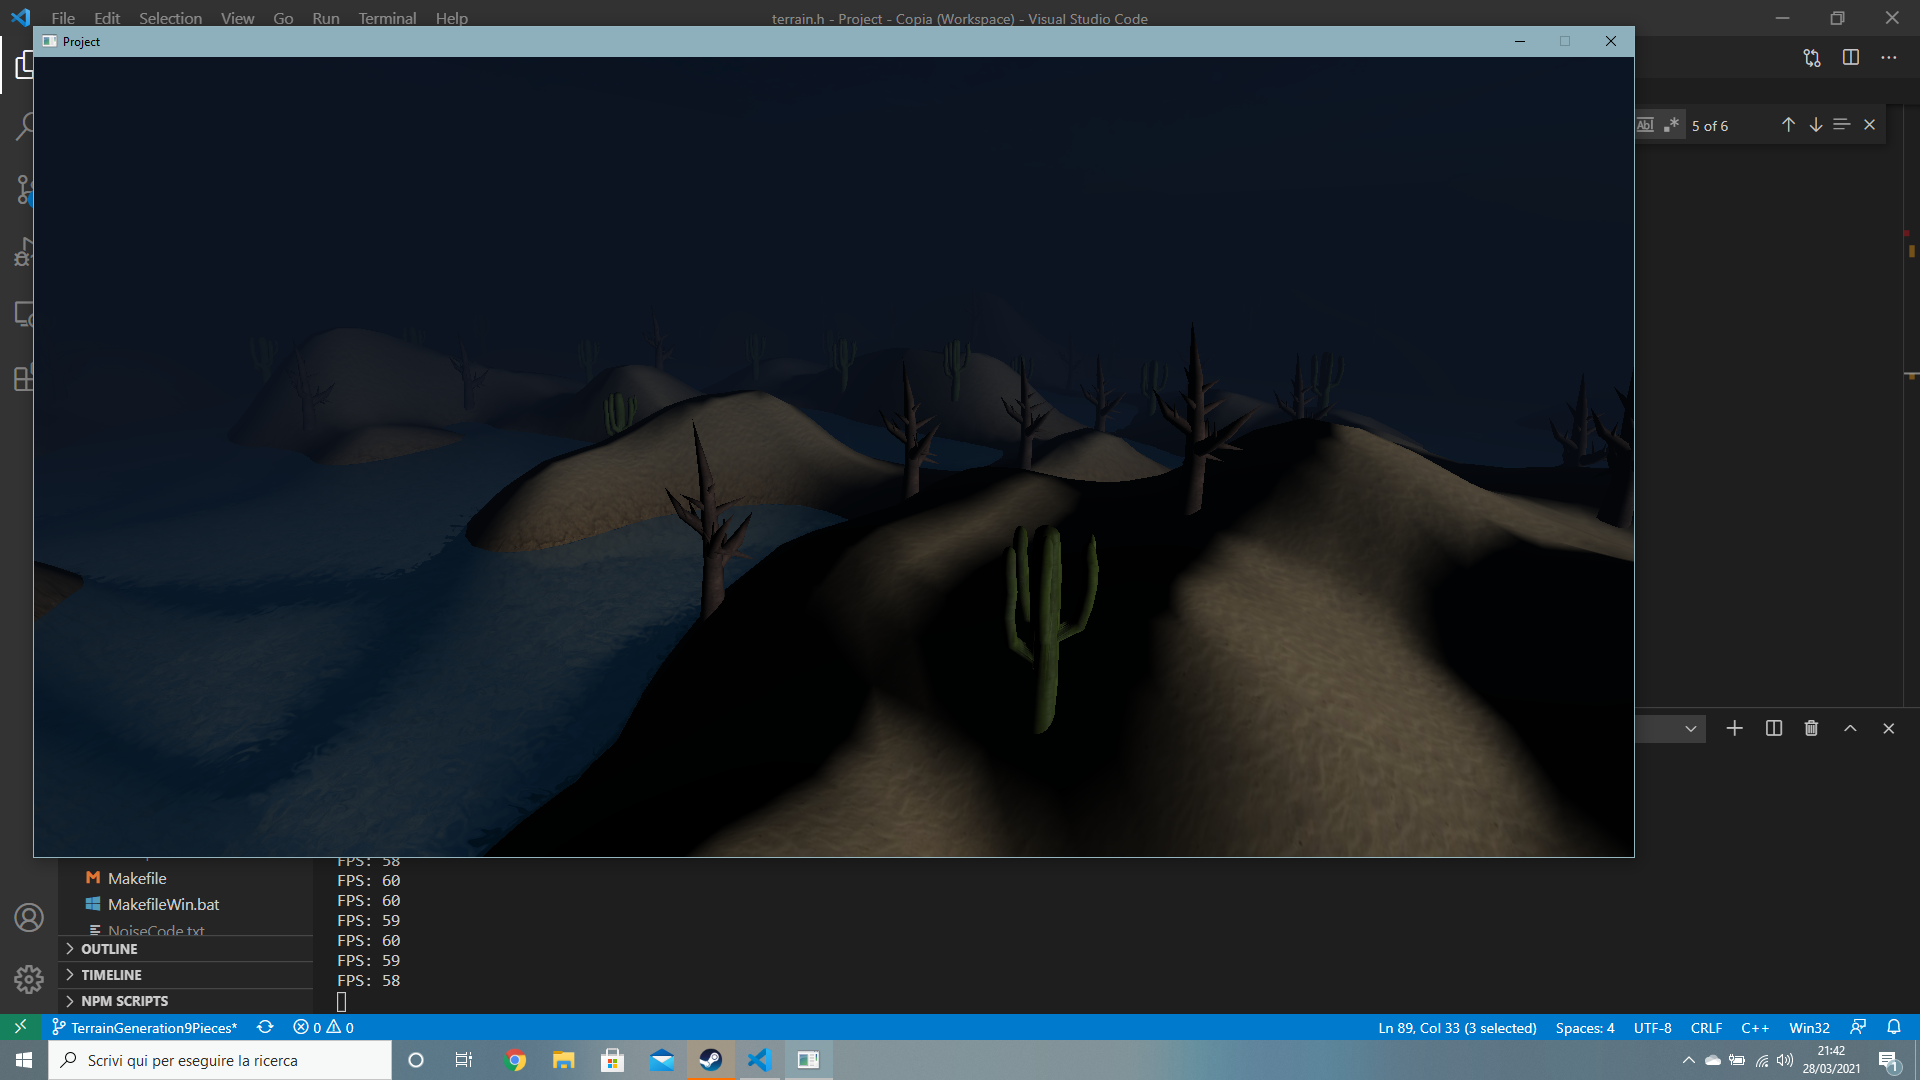
\includegraphics[width=1.4\textwidth,height=0.5\textheight]{images/fps.png}}
	
	\caption{Scene with FPS below. (64-vertices for cell, 441 cells, size 500, height 6000)}
\end{figure} 

\noindent
If I increase the cell size from 500 to 1000/2000 with a height of 12000/18000, the FPS becomes constant at 60 FPS.

\newpage

\begin{figure}[hbt!]
	\centering
	
	\noindent\makebox[\textwidth]{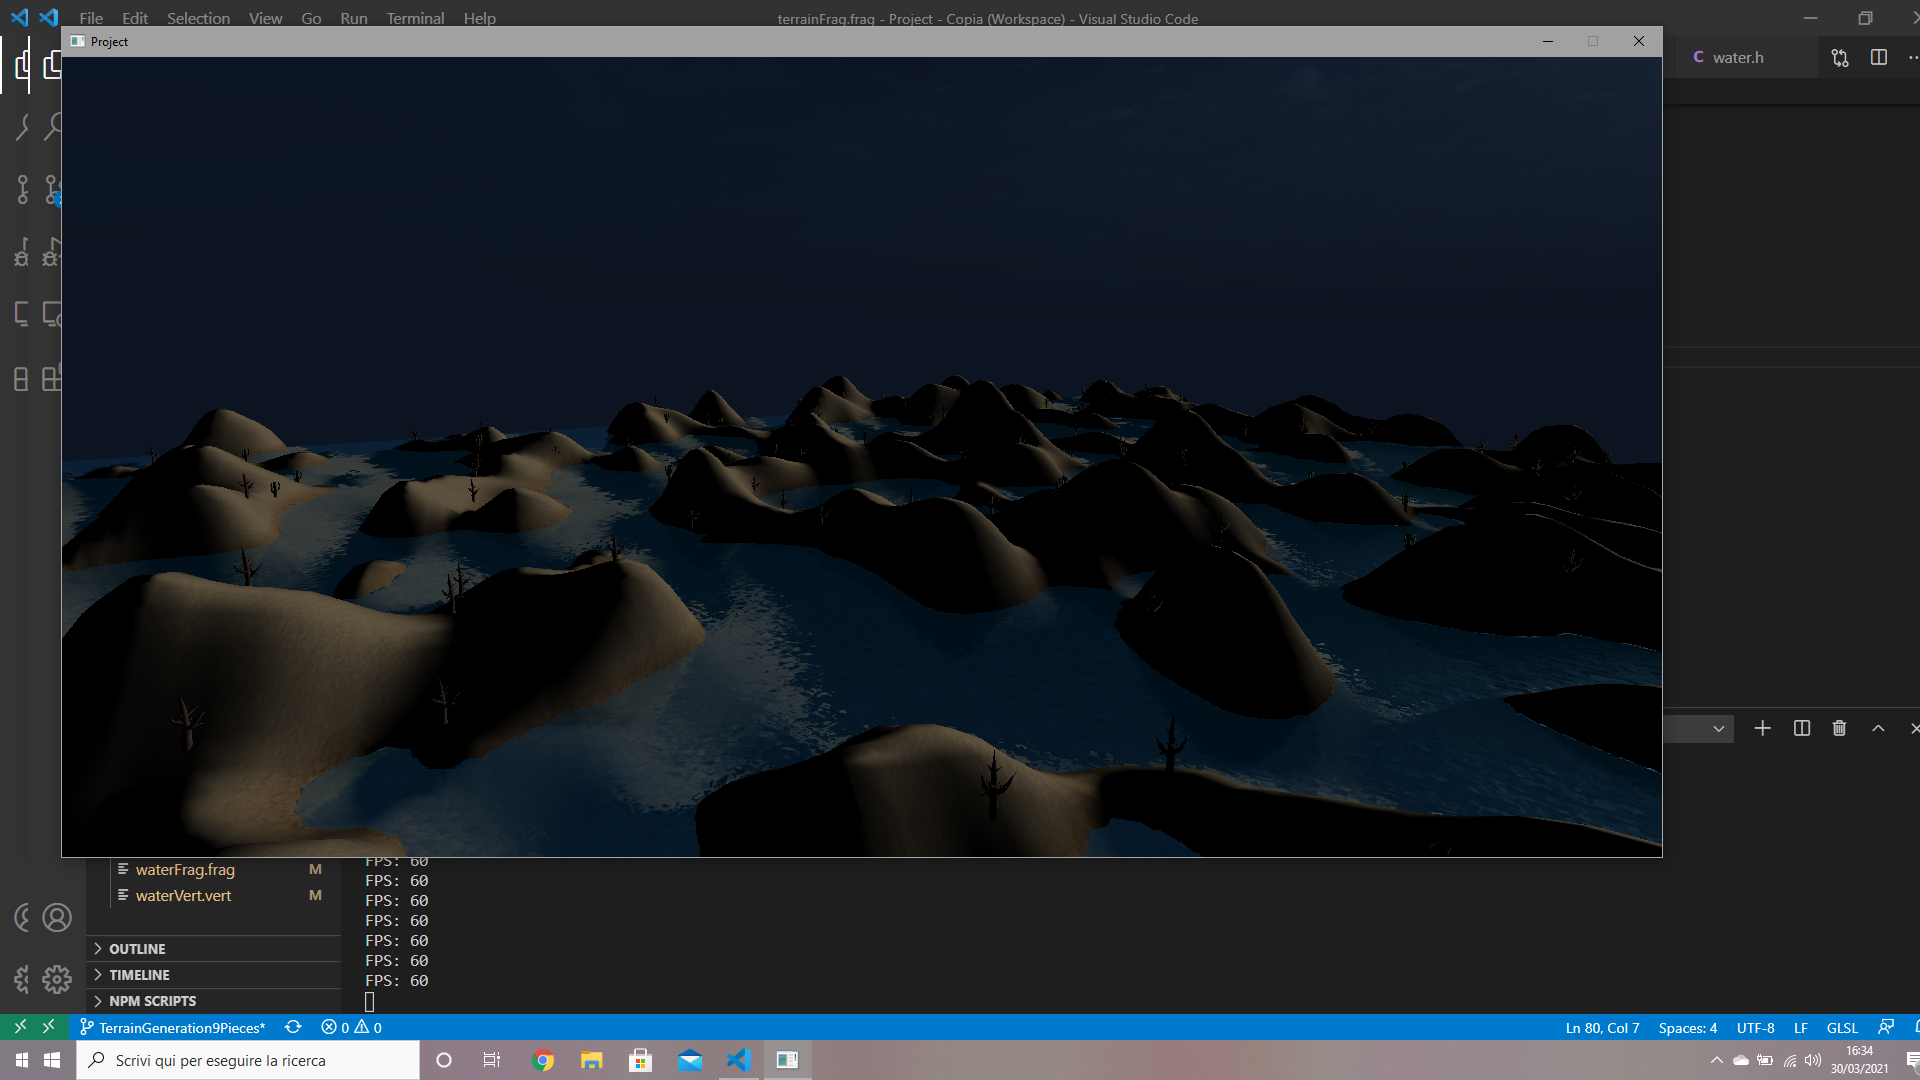
\includegraphics[width=1.4\textwidth,height=0.5\textheight]{images/fps4.png}}
	
	\caption{Scene with FPS below. In this scene I commented the code for the fog in the fragment shaders to let you see that the terrains is really bigger than before. (64-vertices for cell, 441 cells, size 1000, height 12000)}
\end{figure} 

\subsection{16 vertices each row/column}
With 16 vertices, each cell has 256 vertices. If we use 441 cells, we have a total of 112,896 vertices. With a cell size of 500, the scene is rendered with a range between 48 and 50 FPS.

\newpage

\begin{figure}[hbt!]
	\centering
	
	\noindent\makebox[\textwidth]{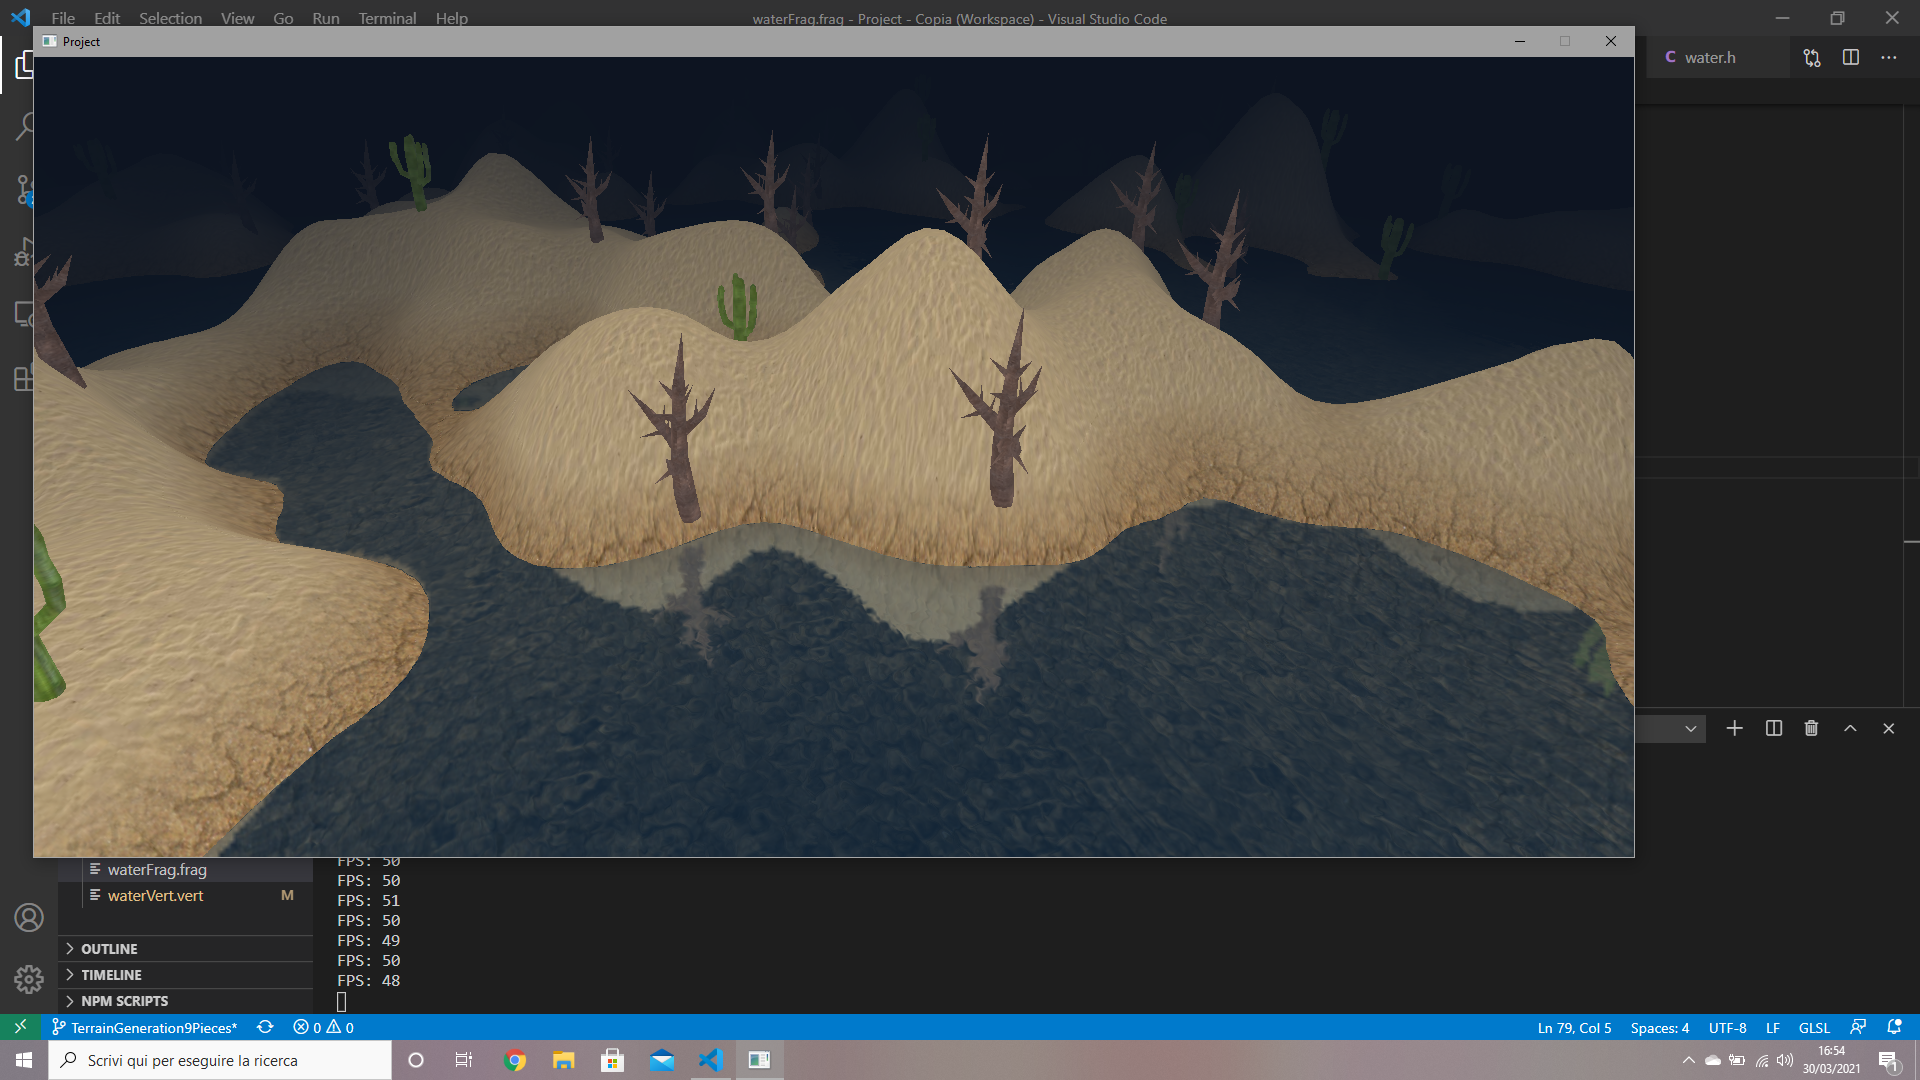
\includegraphics[width=1.4\textwidth,height=0.5\textheight]{images/fps5.png}}
	
	\caption{Scene with FPS below. (256-vertices for cell, 441 cells, size 500, height 3000)}
\end{figure} 

\noindent
I have tried increasing the cell size from 500 to 1000/2000 but the performance is quite similar. So, the solution is to both increase the cell size and decrease the number of cells present in the scene. We now have 21 cells per row, we can change this value to 19 instead and increasing the cell size value to 1000. In this case we now have 361 cells and the scene is rendered with 59 FPS.

\newpage

\begin{figure}[hbt!]
	\centering
	
	\noindent\makebox[\textwidth]{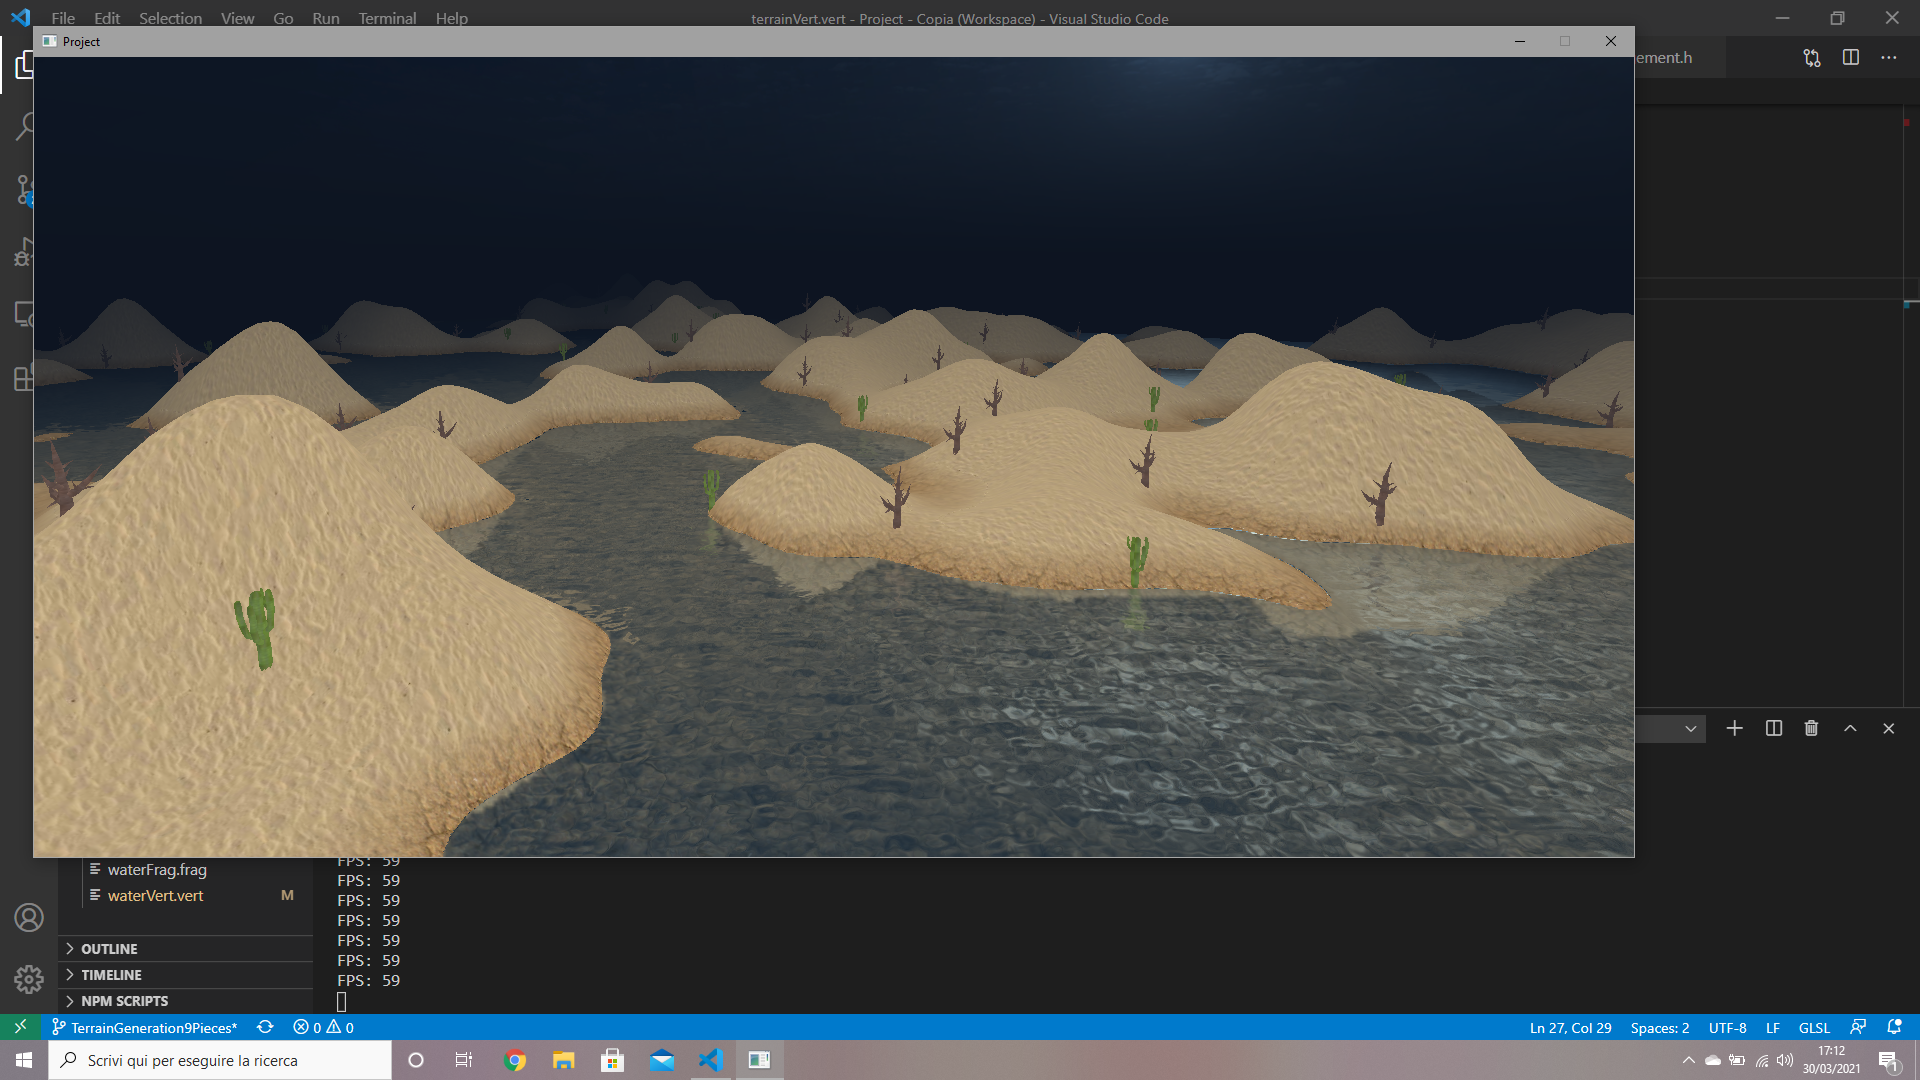
\includegraphics[width=1.4\textwidth,height=0.5\textheight]{images/fps6.png}}
	
	\caption{Scene with FPS below. (256-vertices for cell, 361 cells, size 1000, height 4500)}
\end{figure} 

\subsection{32 vertices each row/column}
With 32 vertices, each cell has 1024 vertices. If we use 441 cells, we have a total of 451,584 vertices. With a cell size of 500, the scene is rendered with 13/14 FPS.

\newpage

\begin{figure}[hbt!]
	\centering
	
	\noindent\makebox[\textwidth]{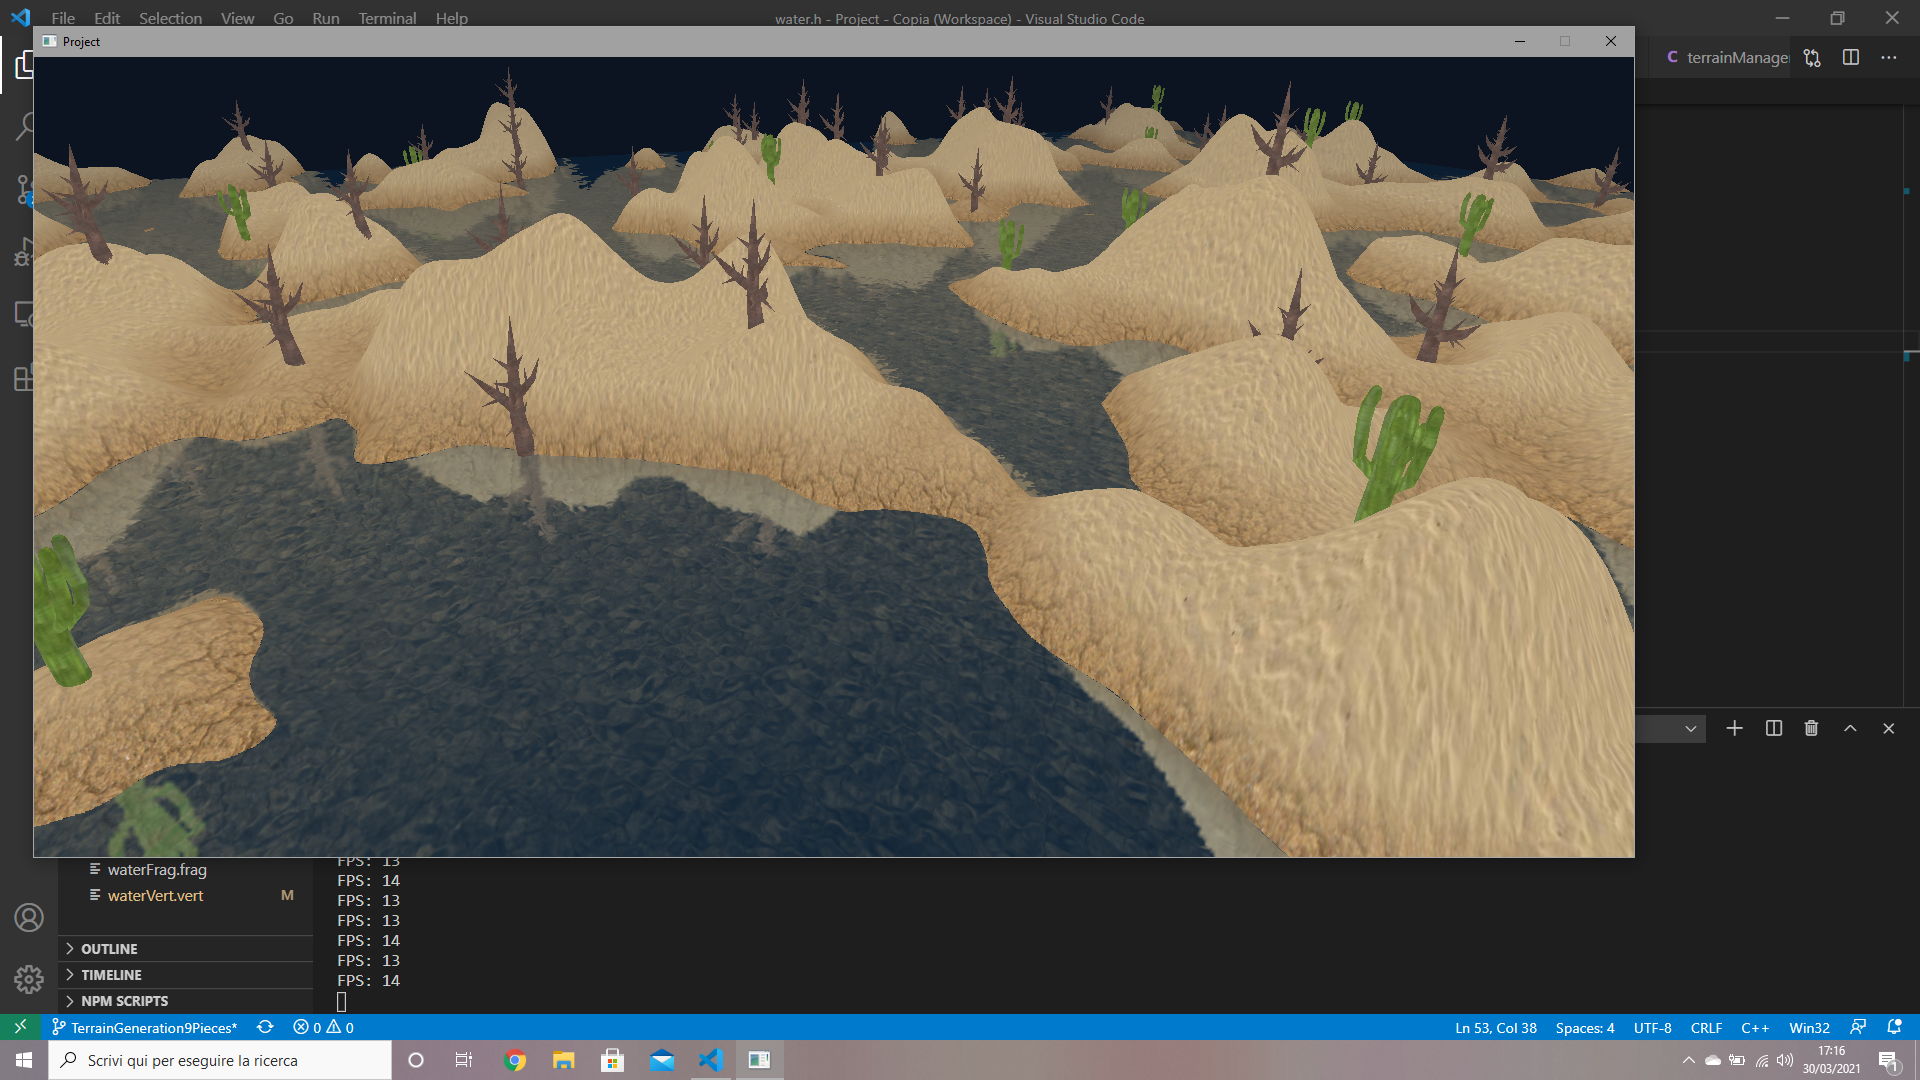
\includegraphics[width=1.4\textwidth,height=0.5\textheight]{images/fps7.png}}
	
	\caption{Scene with FPS below. (1024-vertices for cell, 441 cells, size 500, height 1500)}
\end{figure} 

\noindent
Now I can use the same techniques I used before, increasing the cell size from 500 to 4000 and decreasing the number of cells from 21 to 7. The scene is now rendered at 60 FPS.
\newpage

\begin{figure}[hbt!]
	\centering
	
	\noindent\makebox[\textwidth]{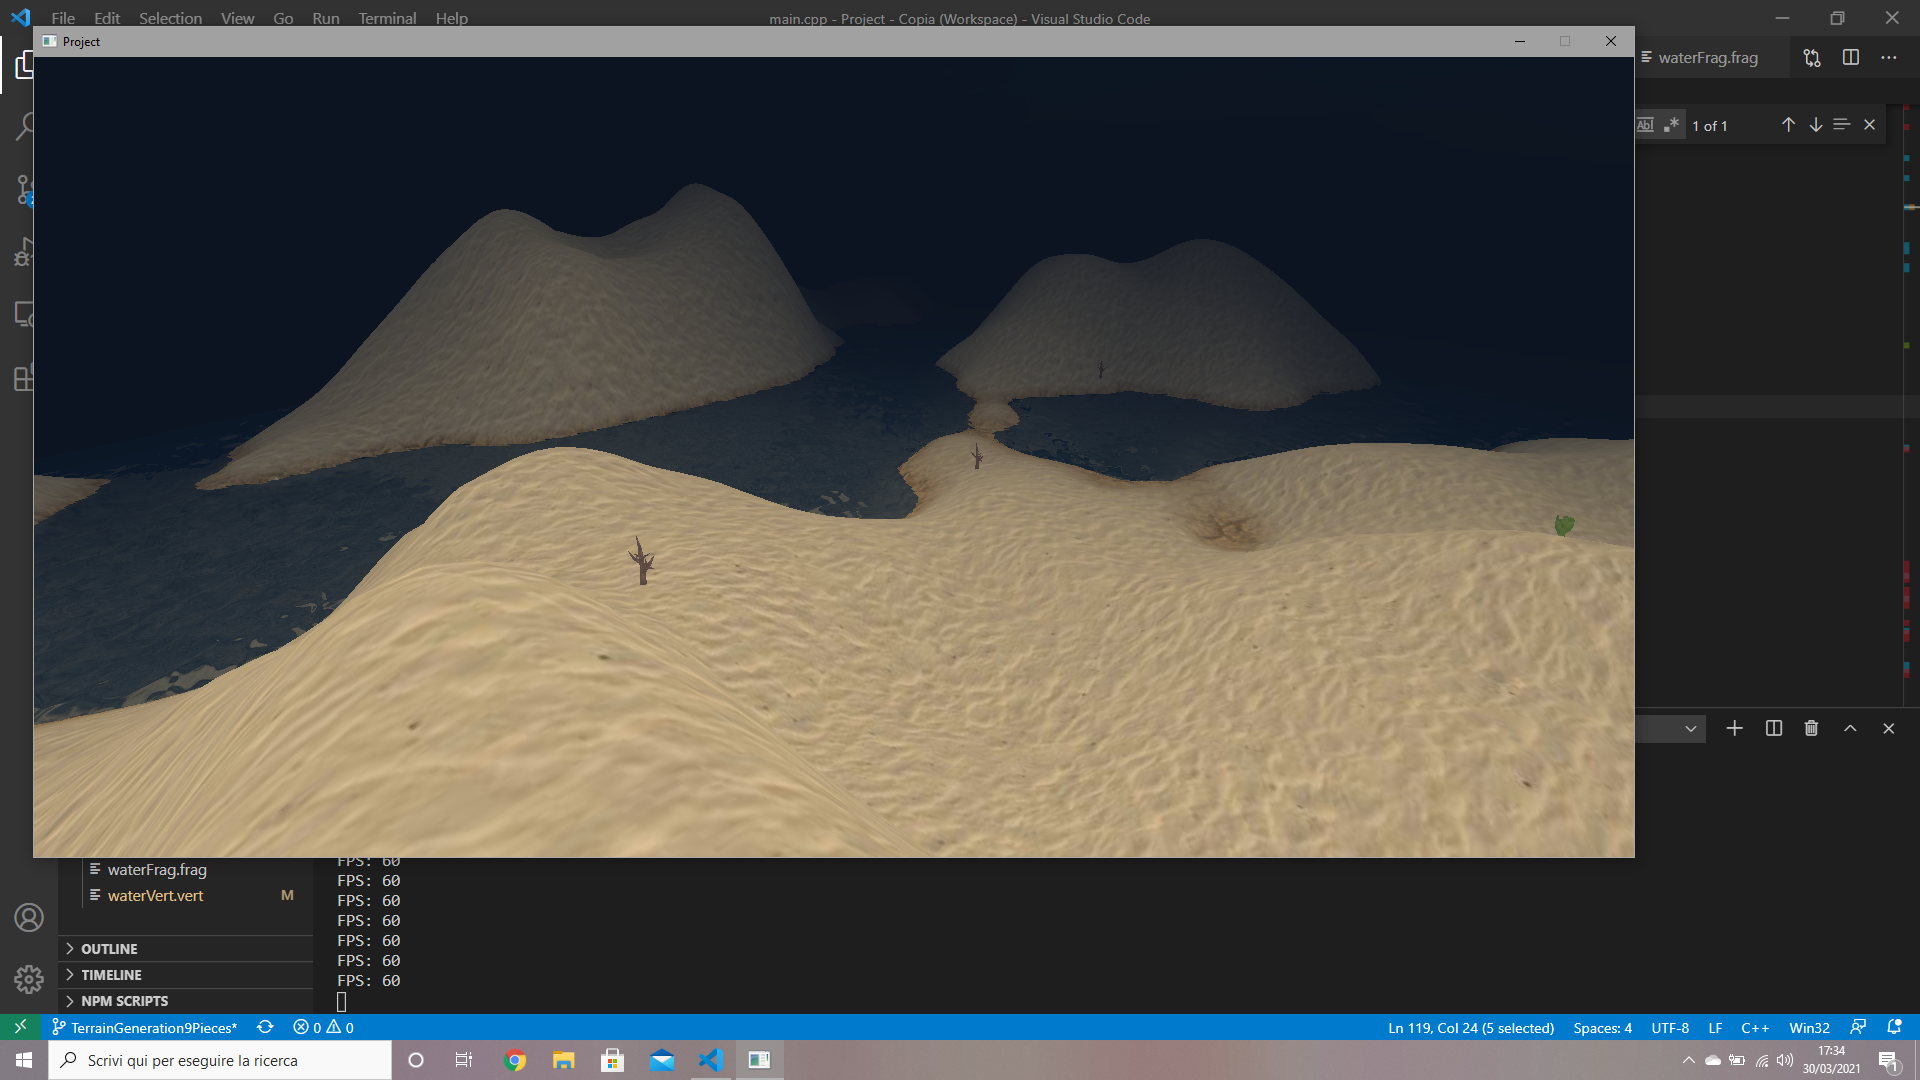
\includegraphics[width=1.4\textwidth,height=0.5\textheight]{images/fps8.png}}
	
	\caption{Scene with FPS below. (1024-vertices for cell, 49 cells, size 4000, height 10000)}
\end{figure} 

\newpage

\begin{figure}[hbt!]
	\centering
	
	\noindent\makebox[\textwidth]{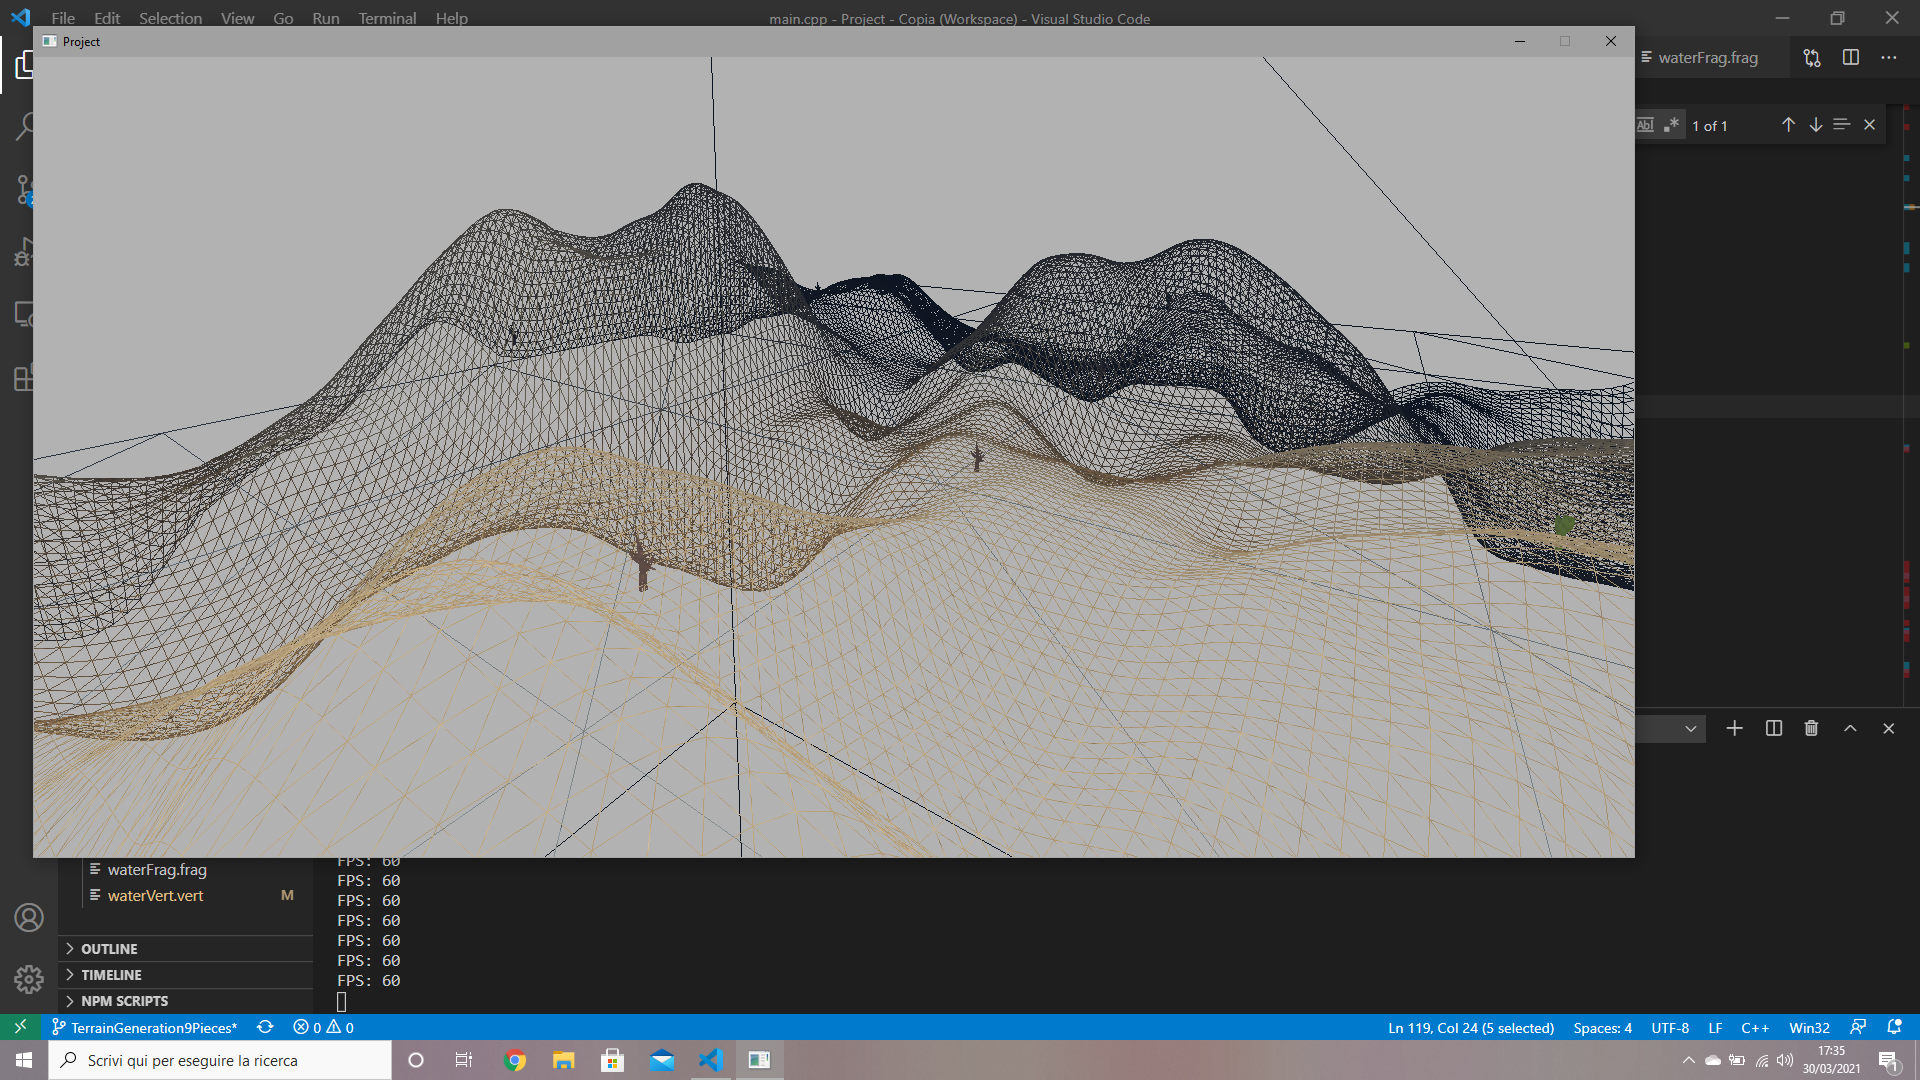
\includegraphics[width=1.4\textwidth,height=0.5\textheight]{images/fps9.png}}
	
	\caption{Same as before but with wireframe active.}
\end{figure} 

\noindent
In the end, I think the terrain is quite flexible since changing the cell size value and the number of vertices I can get different results based on the quality of the terrain.

\newpage

\section{Conclusion}
This is how I implemented everything. If you have any more questions I can answer them during the oral interview.


\begin{figure}[hbt!]
	\centering
	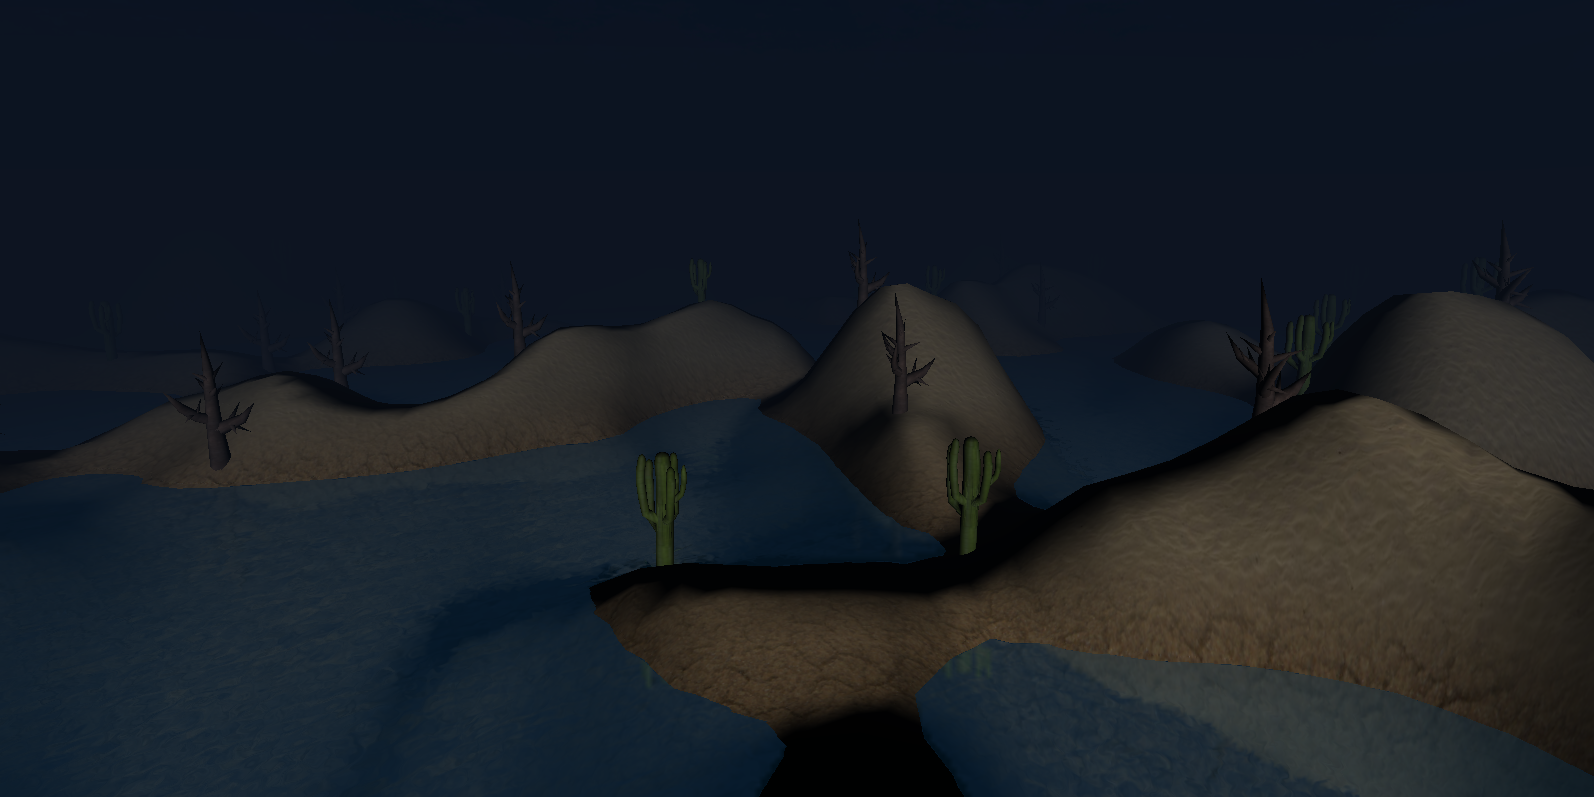
\includegraphics[width= 1
	\textwidth]{images/final1.png}
	\caption{Final image (front view).}
\end{figure}


\begin{figure}[hbt!]
	\centering
	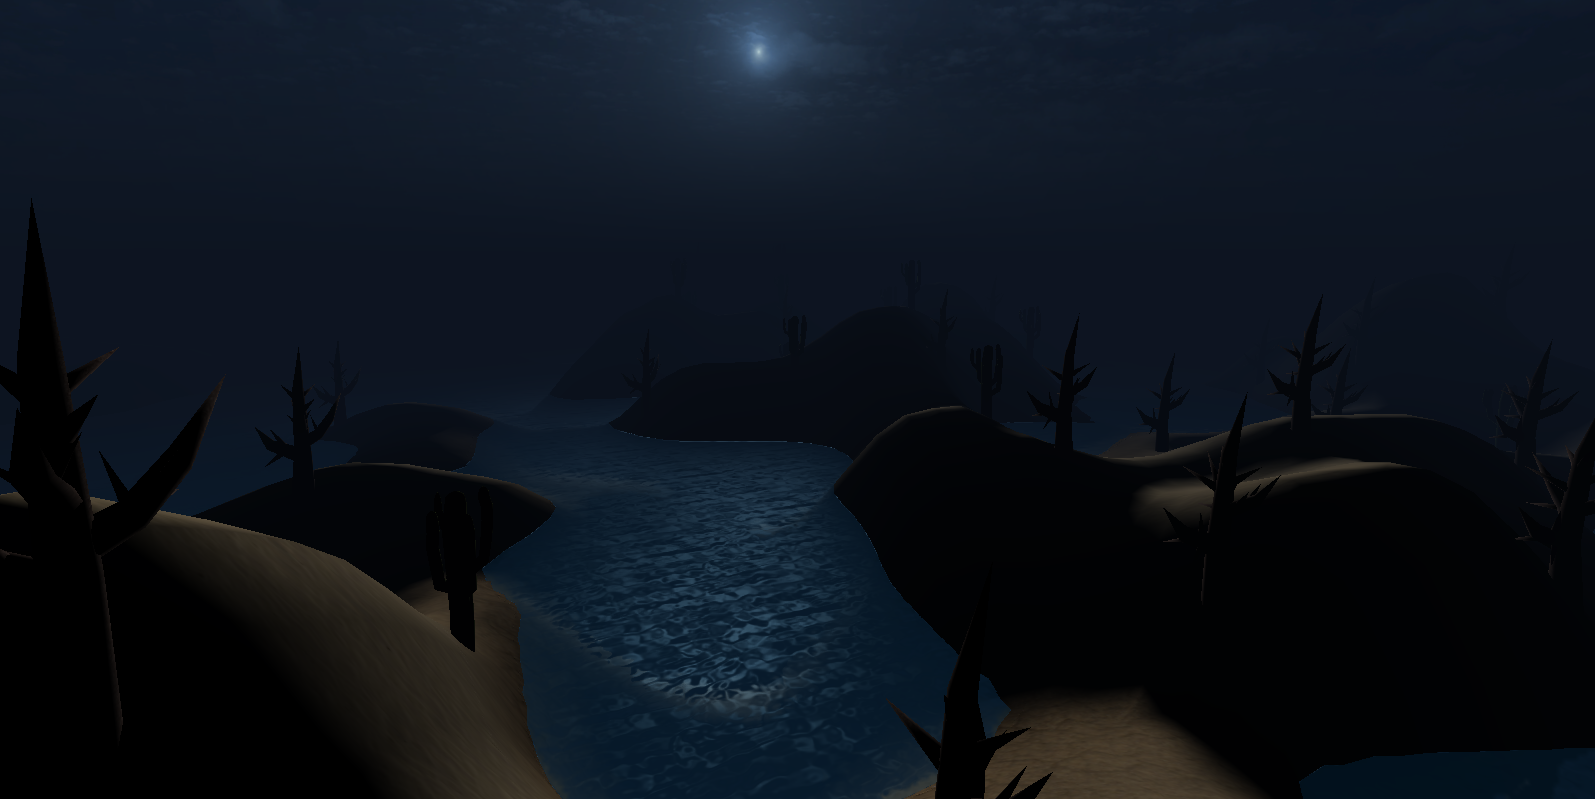
\includegraphics[width= 1
	\textwidth]{images/final2.png}
	\caption{Final image (back view).}
\end{figure}
